% !TEX TS-program = xelatex
% Command for running this example (needs latexmkrc file):
%    latexmk -bibtex -pdf main.tex

%	نمونه پایان‌نامه آماده شده با استفاده از کلاس tehran-thesis، نگارش 1
%	سینا ممکن، دانشگاه تهران 
%	https://github.com/sinamomken/tehran-thesis
%	گروه پارسی‌لاتک
%	http://www.parsilatex.com
%	این نسخه، بر اساس نسخه‌ 0.1 از کلاس IUST-Thesis آقای محمود امین‌طوسی آماده شده است.
%        http://profsite.sttu.ac.ir/mamintoosi

%----------------------------------------------------------------------------------------------
% اگر قصد نوشتن پروژه کارشناسی را دارید، در خط زیر به جای msc، کلمه bsc و اگر قصد نوشتن رساله دکترا را دارید، کلمه phd را قرار دهید. کلیه تنظیمات لازم، به طور خودکار، اعمال می‌شود.

% اگر مایلید پایان‌نامه شما دورو باشد به جای oneside در خط زیر از twoside استفاده کنید.

% برای حاشیه‌نویسی و کم کردن صفحات ابتدایی، گزینه draft را وارد و برای نسخه نهایی آن را حذف کنید.

% برای استفاده از قلم‌های سری IR Series گزینه irfonts را وارد و برای استفاده از قلم‌های X Series 2 آن را حذف کنید.

\documentclass[
twoside
% ,openany
,msc
,irfonts
% ,draft
]{./tex/tehran-thesis}

% فایل commands.tex را مطالعه کنید؛ چون دستورات مربوط به فراخوانی بسته‌ها، فونت و دستورات خاص در این فایل قرار دارد.
% در این فایل، دستورها و تنظیمات مورد نیاز، آورده شده است.
%-------------------------------------------------------------------------------------------------------------------
% دستوراتی که پوشه پیش‌فرض زیرفایل‌های tex را مشخص می‌کند.
%\makeatletter
%\def\input@path{{./tex/}}
%\makeatother
% در ورژن جدید زی‌پرشین برای تایپ متن‌های ریاضی، این سه بسته، حتماً باید فراخوانی شود
\usepackage{amsthm,amssymb,amsmath}
% بسته‌ای برای تنطیم حاشیه‌های بالا، پایین، چپ و راست صفحه
\usepackage[a4paper, top=40mm, bottom=40mm, outer=25mm, inner=35mm]{geometry}
% بسته‌‌ای برای ظاهر شدن شکل‌ها و تعیین آدرس تصاویر
\usepackage[final]{graphicx}
\graphicspath{{./img/}}
% بسته‌های مورد نیاز برای نوشتن کدها، رنگ‌آمیزی آنها و تعیین پوشهٔ کدها
\usepackage[final]{listings}
\usepackage[usenames,dvipsnames,svgnames,table]{xcolor}
\lstset{inputpath=./code/}
% بسته‌ای برای رسم کادر
\usepackage{framed} 
% بسته‌‌ای برای چاپ شدن خودکار تعداد صفحات در صفحه «معرفی پایان‌نامه»
\usepackage{lastpage}
% بسته‌ٔ لازم برای: ۱. تغییر شماره‌گذاری صفحات پیوست. ۲. تصحیح باگ آدرس وب حاوی '%' در مراجع
\usepackage{etoolbox}

%%%%%%%%%%%%%%%%%%%%%%%%%%%%%%%%%%%%
%%% دستورات وابسته به استیل مراجع:
%% اگر از استیل‌های natbib (plainnat-fa، asa-fa، chicago-fa) استفاده می‌کنید، خط زیر را فعال و بعدی‌اش را غیرفعال کنید.
%\usepackage{natbib}
%\newcommand{\citelatin}[1]{\cite{#1}\LTRfootnote{\citeauthor*{#1}}}
%\newcommand{\citeplatin}[1]{\citep{#1}\LTRfootnote{\citeauthor*{#1}}}
%% اگر از سایر استیل‌ها استفاده می‌کنید، خط بالا را غیرفعال و خط‌های زیر را فعال کنید.
\let\citep\cite
\let\citelatin\cite
\let\citeplatin\cite
%%%%%%%%%%%%
% بررسی حالت پیش نویس
\usepackage{ifdraft}
\ifdraft
{%
	% بسته‌ٔ ایجاد لینک‌های رنگی با امکان جهش
	\usepackage[unicode=true,pagebackref=true,
colorlinks,linkcolor=blue,citecolor=blue,final]{hyperref}
	%\usepackage{todonotes}
	\usepackage[firstpage]{draftwatermark}
	\SetWatermarkText{\ \ \ \rl{پیش‌نویس}}
	\SetWatermarkScale{1.2}
}
{ 
	\usepackage[pagebackref=false]{hyperref}
	%\usepackage[disable]{todonotes} % final without TODOs
}

\usepackage[obeyDraft]{todonotes}
\setlength{\marginparwidth}{2cm}

%%%%%%%%%%%%
%%% تصحیح باگ: اگر در مراجع، آدرس وب حاوی '%' بوده و pagebackref فعال باشد، دستورات زیر باید بیایند:
%% برای استیل‌های natbib مثل plainnat-fa، asa-fa، chicago-fa
\makeatletter
\let\ORIG@BR@@lbibitem\BR@@lbibitem
\apptocmd\ORIG@BR@@lbibitem{\endgroup}{}{}
\def\BR@@lbibitem{\begingroup\catcode`\%=12 \ORIG@BR@@lbibitem}
\makeatother
%% برای سایر استیل‌ها
\makeatletter
\let\ORIG@BR@@bibitem\BR@@bibitem
\apptocmd\ORIG@BR@@bibitem{\endgroup}{}{}
\def\BR@@bibitem{\begingroup\catcode`\%=12 \ORIG@BR@@bibitem}
\makeatother
%%%%%%%%%%%%%%%%%%%%%%%%%%%%%%%%%%%%

% بسته‌ لازم برای تنظیم سربرگ‌ها
\usepackage{fancyhdr}
%\usepackage{enumitem}
\usepackage{setspace}
% بسته‌های لازم برای نوشتن الگوریتم
\usepackage{algorithm}
\usepackage{algorithmic}
% بسته‌های لازم برای رسم بهتر جداول
\usepackage{tabulary}
\usepackage{tabularx}
\usepackage{rotating}
% بسته‌های لازم برای رسم تنظیم بهتر شکل‌ها و زیرشکل‌ها
\usepackage[export]{adjustbox}
\usepackage{subfig}
\usepackage[subfigure]{tocloft}
% بسته‌ای برای رسم نمودارها و نیز صفحه مالکیت اثر
\usepackage{tikz}
% بسته‌ای برای ظاهر شدن «مراجع» و «نمایه» در فهرست مطالب
\usepackage[nottoc]{tocbibind}
% دستورات مربوط به ایجاد نمایه
\usepackage{makeidx}
\makeindex
%%% بسته ایجاد واژه‌نامه با xindy
\usepackage[xindy,toc,acronym,nonumberlist=true]{glossaries}

% بسته‌ای برای افزودن تورفتگی به ابتدای اولین پاراگراف هر بخش
\usepackage{indentfirst}

% بسته زیر باگ ناشی از فراخوانی بسته‌های زیاد را برطرف می‌کند.
\usepackage{morewrites}
%%%%%%%%%%%%%%%%%%%%%%%%%%
% فراخوانی بسته زی‌پرشین (باید آخرین بسته باشد)
\usepackage[extrafootnotefeatures, localise=on, displaymathdigits=persian]{xepersian}




\makeatletter
% تعریف قلم فارسی و انگلیسی و مکان قلم‌ها
\if@irfonts
\settextfont[Path={./font/}, BoldFont={IRLotusICEE_Bold.ttf}, BoldItalicFont={IRLotusICEE_BoldIranic.ttf}, ItalicFont={IRLotusICEE_Iranic.ttf},Scale=1.2]{IRLotusICEE.ttf}
% LiberationSerif or FreeSerif as free equivalents of Times New Roman
\setlatintextfont[Path={./font/}, BoldFont={LiberationSerif-Bold.ttf}, BoldItalicFont={LiberationSerif-BoldItalic.ttf}, ItalicFont={LiberationSerif-Italic.ttf},Scale=1]{LiberationSerif-Regular.ttf}
% چنانچه می‌خواهید اعداد در فرمول‌ها، انگلیسی باشد، خط زیر را غیرفعال کنید
% و گزینهٔ displaymathdigits=persian را از خط ۱۰۹ حذف کنید.
\setdigitfont[Path={./font/}, Scale=1.2]{IRLotusICEE.ttf}
% تعریف قلم‌های فارسی و انگلیسی اضافی برای استفاده در بعضی از قسمت‌های متن
\setiranicfont[Path={./font/}, Scale=1.3]{IRLotusICEE_Iranic.ttf}				% ایرانیک، خوابیده به چپ
\setmathsfdigitfont[Path={./font/}]{IRTitr.ttf}
\defpersianfont\titlefont[Path={./font/}, Scale=1]{IRTitr.ttf}
% برای تعریف یک قلم خاص عنوان لاتین، خط بعد را فعال و ویرایش کنید و خط بعد از آن را غیرفعال کنید.
% \deflatinfont\latintitlefont[Scale=1]{LiberationSerif}
\font\latintitlefont=cmssbx10 scaled 2300 %cmssbx10 scaled 2300
\else
\settextfont{XB Niloofar}
\setlatintextfont{Junicode}
% چنانچه می‌خواهید اعداد در فرمول‌ها، انگلیسی باشد، خط زیر را غیرفعال کنید
% و گزینهٔ displaymathdigits=persian را از خط ۱۰۹ حذف کنید.
\setdigitfont{XB Niloofar}
% تعریف قلم‌های فارسی و انگلیسی اضافی برای استفاده در بعضی از قسمت‌های متن
% \setmathsfdigitfont{XB Titre}
\defpersianfont\titlefont{XB Titre}
\deflatinfont\latintitlefont[Scale=1.1]{Junicode}
\fi
\makeatother

% برای استفاده از قلم نستعلیق خط بعد را فعال کنید.
% \defpersianfont\nastaliq[Scale=1.2]{IranNastaliq}


%%%%%%%%%%%%%%%%%%%%%%%%%%
% راستچین شدن todonotes
\presetkeys{todonotes}{align=right,textdirection=righttoleft}{}
\makeatletter
\providecommand\@dotsep{5}
\def\listtodoname{فهرست کارهای باقیمانده}
\def\listoftodos{\noindent{\Large\vspace{10mm}\textbf{\listtodoname}}\@starttoc{tdo}}
\renewcommand{\@todonotes@MissingFigureText}{شکل}
\renewcommand{\@todonotes@MissingFigureUp}{شکل}
\renewcommand{\@todonotes@MissingFigureDown}{جاافتاده}
\makeatother
% دستوری برای حذف کلمه «چکیده»
% \renewcommand{\abstractname}{}
% دستوری برای حذف کلمه «abstract»
%\renewcommand{\latinabstract}{}
% دستوری برای تغییر نام کلمه «اثبات» به «برهان»
\renewcommand\proofname{\textbf{برهان}}
% دستوری برای تغییر نام کلمه «کتاب‌نامه» به «مراجع»
\renewcommand{\bibname}{مراجع}
% دستوری برای تعریف واژه‌نامه انگلیسی به فارسی
\newcommand\persiangloss[2]{#1\dotfill\lr{#2}\\}
% دستوری برای تعریف واژه‌نامه فارسی به انگلیسی 
\newcommand\englishgloss[2]{#2\dotfill\lr{#1}\\}
% تعریف دستور جدید «\پ» برای خلاصه‌نویسی جهت نوشتن عبارت «پروژه/پایان‌نامه/رساله»
\newcommand{\پ}{پروژه/پایان‌نامه/رساله }

%\newcommand\BackSlash{\char`\\}

%%%%%%%%%%%%%%%%%%%%%%%%%%
% \SepMark{-}

% تعریف و نحوه ظاهر شدن عنوان قضیه‌ها، تعریف‌ها، مثال‌ها و ...
\theoremstyle{definition}
\newtheorem{definition}{تعریف}[section]
\theoremstyle{theorem}
\newtheorem{theorem}[definition]{قضیه}
\newtheorem{lemma}[definition]{لم}
\newtheorem{proposition}[definition]{گزاره}
\newtheorem{corollary}[definition]{نتیجه}
\newtheorem{remark}[definition]{ملاحظه}
\theoremstyle{definition}
\newtheorem{example}[definition]{مثال}

%\renewcommand{\theequation}{\thechapter-\arabic{equation}}
%\def\bibname{مراجع}
\numberwithin{algorithm}{chapter}
\def\listalgorithmname{فهرست الگوریتم‌ها}
\def\listfigurename{فهرست تصاویر}
\def\listtablename{فهرست جداول}

% دستور های لازم برای تعریف ترجمهٔ دستورات الگوریتم
\makeatletter
\renewcommand{\algorithmicrequire}{\if@RTL\textbf{ورودی:}\else\textbf{Require:}\fi}
\renewcommand{\algorithmicensure}{\if@RTL\textbf{خروجی:}\else\textbf{Ensure:}\fi}
\renewcommand{\algorithmicend}{\if@RTL\textbf{پایان}\else\textbf{end}\fi}
\renewcommand{\algorithmicif}{\if@RTL\textbf{اگر}\else\textbf{if}\fi}
\renewcommand{\algorithmicthen}{\if@RTL\textbf{آنگاه}\else\textbf{then}\fi}
\renewcommand{\algorithmicelse}{\if@RTL\textbf{وگرنه}\else\textbf{else}\fi}
\renewcommand{\algorithmicfor}{\if@RTL\textbf{برای}\else\textbf{for}\fi}
\renewcommand{\algorithmicforall}{\if@RTL\textbf{برای هر}\else\textbf{for all}\fi}
\renewcommand{\algorithmicdo}{\if@RTL\textbf{انجام بده}\else\textbf{do}\fi}
\renewcommand{\algorithmicwhile}{\if@RTL\textbf{تا زمانی که}\else\textbf{while}\fi}
\renewcommand{\algorithmicloop}{\if@RTL\textbf{تکرار کن}\else\textbf{loop}\fi}
\renewcommand{\algorithmicrepeat}{\if@RTL\textbf{تکرار کن}\else\textbf{repeat}\fi}
\renewcommand{\algorithmicuntil}{\if@RTL\textbf{تا زمانی که}\else\textbf{until}\fi}
\renewcommand{\algorithmicprint}{\if@RTL\textbf{چاپ کن}\else\textbf{print}\fi}
\renewcommand{\algorithmicreturn}{\if@RTL\textbf{بازگردان}\else\textbf{return}\fi}
\renewcommand{\algorithmicand}{\if@RTL\textbf{و}\else\textbf{and}\fi}
\renewcommand{\algorithmicor}{\if@RTL\textbf{و یا}\else\textbf{or}\fi} % TODO add better translate
\renewcommand{\algorithmicxor}{\if@RTL\textbf{یا}\else\textbf{xor}\fi} % TODO add better translate
\renewcommand{\algorithmicnot}{\if@RTL\textbf{نقیض}\else\textbf{not}\fi}
\renewcommand{\algorithmicto}{\if@RTL\textbf{تا}\else\textbf{to}\fi}
\renewcommand{\algorithmicinputs}{\if@RTL\textbf{ورودی‌ها}\else\textbf{inputs}\fi}
\renewcommand{\algorithmicoutputs}{\if@RTL\textbf{خروجی‌ها}\else\textbf{outputs}\fi}
\renewcommand{\algorithmicglobals}{\if@RTL\textbf{متغیرهای عمومی}\else\textbf{globals}\fi}
\renewcommand{\algorithmicbody}{\if@RTL\textbf{انجام بده}\else\textbf{do}\fi}
\renewcommand{\algorithmictrue}{\if@RTL\textbf{درست}\else\textbf{true}\fi}
\renewcommand{\algorithmicfalse}{\if@RTL\textbf{نادرست}\else\textbf{false}\fi}
\renewcommand{\algorithmicendif}{\algorithmicend\textbf{ شرط }\algorithmicif}
\renewcommand{\algorithmicendfor}{\algorithmicend\textbf{ حلقهٔ }\algorithmicfor}
\renewcommand{\algorithmicendwhile}{\algorithmicend\textbf{ حلقهٔ }\algorithmicwhile}
\renewcommand{\algorithmicendloop}{\algorithmicend\textbf{ حلقهٔ }\algorithmicloop}
\renewcommand{\algorithmiccomment}[1]{\{{\itshape #1}\}}
\makeatletter

%%%%%%%%%%%%%%%%%%%%%%%%%%%%
%%% دستورهایی برای سفارشی کردن سربرگ صفحات:
%\newcommand{\SetHeader}[1]{
% دستور زیر معادل با گزینه twoside است.
%\csname@twosidetrue\endcsname
\pagestyle{fancy}
%% دستورات زیر سبک صفحات fancy را تغییر می‌دهد:
% O=Odd, E=Even, L=Left, R=Right
% در صورت oneside بودن، عنوان فصل، سمت چپ ظاهر می‌شود.
\fancyhead{}
\fancyhead[OL]{\small\leftmark}
\fancyhead[ER]{\small\leftmark}
\fancyhead[OR]{\footnotesize\rightmark}
\fancyhead[EL]{\footnotesize\rightmark}
\renewcommand{\headrulewidth}{0.75pt}
% شکل‌دهی شماره و عنوان فصل در سربرگ
\renewcommand{\chaptermark}[1]{\markboth{\@chapapp~\thechapter:\ #1}{}}
\makeatletter
\renewcommand{\rightmark}[1]{\@title}
\makeatother
%}
%%%%%%%%%%%%%%%%%%%%%%%%%%%%
%\def\MATtextbaseline{1.5}
%\renewcommand{\baselinestretch}{\MATtextbaseline}
\doublespacing
%%%%%%%%%%%%%%%%%%%%%%%%%%%%%
% دستوراتی برای اضافه کردن کلمه «فصل» در فهرست مطالب

\newlength\mylenprt
\newlength\mylenchp
\newlength\mylenapp

\renewcommand\cftpartpresnum{\partname~}
\renewcommand\cftchappresnum{\chaptername~}
\renewcommand\cftchapaftersnum{:}

\settowidth\mylenprt{\cftpartfont\cftpartpresnum\cftpartaftersnum}
\settowidth\mylenchp{\cftchapfont\cftchappresnum\cftchapaftersnum}
\settowidth\mylenapp{\cftchapfont\appendixname~\cftchapaftersnum}
\addtolength\mylenprt{\cftpartnumwidth}
\addtolength\mylenchp{\cftchapnumwidth}
\addtolength\mylenapp{\cftchapnumwidth}

\setlength\cftpartnumwidth{\mylenprt}
\setlength\cftchapnumwidth{\mylenchp}	

\makeatletter
{\def\thebibliography#1{\chapter*{\refname\@mkboth
   {\uppercase{\refname}}{\uppercase{\refname}}}\list
   {[\arabic{enumi}]}{\settowidth\labelwidth{[#1]}
   \rightmargin\labelwidth
   \advance\rightmargin\labelsep
   \advance\rightmargin\bibindent
   \itemindent -\bibindent

   \listparindent \itemindent
   \parsep \z@
   \usecounter{enumi}}
   \def\newblock{}
   \sloppy
   \sfcode`\.=1000\relax}}
   
%اگر مایلید در شماره گذاری حرفی و ابجد به جای آ از الف استفاده شود دستورات زیر را فعال کنید.   
%\def\@Abjad#1{%
%  \ifcase#1\or الف\or ب\or ج\or د%
%           \or هـ\or و\or ز\or ح\or ط%
%           \or ی\or ک\or ل\or م\or ن%
%           \or س\or ع\or ف\or ص%
%           \or ق\or ر\or ش\or ت\or ث%
%            \or خ\or ذ\or ض\or ظ\or غ%
%            \else\@ctrerr\fi}
%
% \def\abj@num@i#1{%
%   \ifcase#1\or الف\or ب\or ج\or د%
%            \or هـ‍\or و\or ز\or ح\or ط\fi

%   \ifnum#1=\z@\abjad@zero\fi}   
%  
%   \def\@harfi#1{\ifcase#1\or الف\or ب\or پ\or ت\or ث\or

% ج\or چ\or ح\or خ\or د\or ذ\or ر\or ز\or ژ\or س\or ش\or ص\or ض\or ط\or ظ\or ع\or غ\or

% ف\or ق\or ک\or گ\or ل\or م\or ن\or و\or ه\or ی\else\@ctrerr\fi}

%
\makeatother

%%% امکان درج کد در سند
% در این قسمت رنگ، قلم و قالب‌بندی قسمت‌های مختلف یک کد تعیین می‌شود. 
\lstdefinestyle{myStyle}{
	basicstyle=\ttfamily, % whole listing /w verbatim font
	keywordstyle=\color{blue}\bfseries, % bold black keywords
	identifierstyle=, % nothing happens
	commentstyle=\color{LimeGreen}, % green comments
	stringstyle=\ttfamily\color{red}, % red typewriter font for strings
	showstringspaces=false % no special string spaces
	breaklines=true,
	breakatwhitespace=false,
	numbers=right, % line number formats
	numberstyle=\footnotesize\lr,
	numbersep=-10pt,
	frame=single,
	captionpos=b,
	captiondirection=RTL
}
\lstset{style=myStyle} % command to set default style
\def\lstlistingname{\rl{برنامهٔ}}
\def\lstlistlistingname{\rl{فهرست برنامه‌ها}}


% for numbering subsubsections
\setcounter{secnumdepth}{3}
%to include subsubsections in the table of contents
\setcounter{tocdepth}{3}

\makeatletter
\renewcommand{\p@subfigure}{\thefigure.}
\makeatother


% مشخصات پایان‌نامه را در فایلهای faTitle و enTitle وارد نمایید.
% !TeX root=../main.tex
% در این فایل، عنوان پایان‌نامه، مشخصات خود، متن تقدیمی‌، ستایش، سپاس‌گزاری و چکیده پایان‌نامه را به فارسی، وارد کنید.
% توجه داشته باشید که جدول حاوی مشخصات پروژه/پایان‌نامه/رساله و همچنین، مشخصات داخل آن، به طور خودکار، درج می‌شود.
%%%%%%%%%%%%%%%%%%%%%%%%%%%%%%%%%%%%
% دانشگاه خود را وارد کنید
\university{دانشگاه تهران}
% پردیس دانشگاهی خود را اگر نیاز است وارد کنید (مثال: فنی، علوم پایه، علوم انسانی و ...)
\college{پردیس دانشکده‌های فنی}
% دانشکده، آموزشکده و یا پژوهشکده  خود را وارد کنید
\faculty{دانشکده‌ی مهندسی برق و کامپیوتر}
% گروه آموزشی خود را وارد کنید (در صورت نیاز)
\department{گروه شبکه و سیستم‌های امن}
% رشته تحصیلی خود را وارد کنید
%\subject{مهندسی برق}
% گرایش خود را وارد کنید
%\field{شبکه‌های مخابراتی}
% عنوان پایان‌نامه را وارد کنید
\title{استراتژی ذخیرە‌سازی در شبکه‌های اینترنت اشیا براساس یادگیری تقویتی عمیق}
% نام استاد(ان) راهنما را وارد کنید
\firstsupervisor{دکتر ناصر یزدانی}
\firstsupervisorrank{استاد}
\secondsupervisor{دکتر سید پویا شریعت پناهی}
\secondsupervisorrank{استاد}
% نام استاد(دان) مشاور را وارد کنید. چنانچه استاد مشاور ندارید، دستورات پایین را غیرفعال کنید.
%\firstadvisor{دکتر مشاور اول}
%\firstadvisorrank{استادیار}
%\secondadvisor{دکتر مشاور دوم}
% نام داوران داخلی و خارجی خود را وارد نمایید.
%\internaljudge{دکتر داور داخلی}
%\internaljudgerank{دانشیار}
%\externaljudge{دکتر داور خارجی}
%\externaljudgerank{دانشیار}
%\externaljudgeuniversity{دانشگاه داور خارجی}
% نام نماینده کمیته تحصیلات تکمیلی در دانشکده \ گروه
%\graduatedeputy{دکتر نماینده}
%\graduatedeputyrank{دانشیار}
% نام دانشجو را وارد کنید
\name{تابان}
% نام خانوادگی دانشجو را وارد کنید
\surname{سلیمانی}
% شماره دانشجویی دانشجو را وارد کنید
\studentID{810100377}
% تاریخ پایان‌نامه را وارد کنید
\thesisdate{دی 1401}
% به صورت پیش‌فرض برای پایان‌نامه‌های کارشناسی تا دکترا به ترتیب از عبارات «پروژه»، «پایان‌نامه» و «رساله» استفاده می‌شود؛ اگر  نمی‌پسندید هر عنوانی را که مایلید در دستور زیر قرار داده و آنرا از حالت توضیح خارج کنید.
\projectLabel{گزارش نهایی درس سمینار}

% به صورت پیش‌فرض برای عناوین مقاطع تحصیلی کارشناسی تا دکترا به ترتیب از عبارت «کارشناسی»، «کارشناسی ارشد» و «دکتری» استفاده می‌شود؛ اگر نمی‌پسندید هر عنوانی را که مایلید در دستور زیر قرار داده و آنرا از حالت توضیح خارج کنید.
%\degree{ن}
%%%%%%%%%%%%%%%%%%%%%%%%%%%%%%%%%%%%%%%%%%%%%%%%%%%%
%% پایان‌نامه خود را تقدیم کنید! %%
\dedication
{
{\Large تقدیم به:}\\
\begin{flushleft}{
	\huge
	همسر و فرزندانم\\
	\vspace{7mm}
	و\\
	\vspace{7mm}
	پدر و مادرم
}
\end{flushleft}
}
%% متن قدردانی %%
%% ترجیحا با توجه به ذوق و سلیقه خود متن قدردانی را تغییر دهید.
\acknowledgement{
سپاس خداوندگار حکیم را که با لطف بی‌کران خود، آدمی را به زیور عقل آراست.

در آغاز وظیفه‌  خود  می‌دانم از زحمات بی‌دریغ اساتید  راهنمای خود،  جناب آقای دکتر ... و ...، صمیمانه تشکر و  قدردانی کنم که در طول انجام این پایان‌نامه با نهایت صبوری همواره راهنما و مشوق من بودند و قطعاً بدون راهنمایی‌های ارزنده‌ ایشان، این مجموعه به انجام نمی‌رسید.

از جناب آقای دکتر ... که  زحمت مشاوره‌، بازبینی و تصحیح این پایان‌نامه را تقبل فرمودند کمال امتنان را دارم.

%از همکاری و مساعدت‌های دکتر ... مسئول تحصیلات تکمیلی و سایر کارکنان دانشکده بویژه سرکار خانم ... کمال تشکر را دارم.

با سپاس بی‌دریغ خدمت دوستان گران‌مایه‌ام، خانم‌ها ... و آقایان ... در آزمایشگاه ...، که با همفکری مرا صمیمانه و مشفقانه یاری داده‌اند.

و در پایان، بوسه می‌زنم بر دستان خداوندگاران مهر و مهربانی، پدر و مادر عزیزم و بعد از خدا، ستایش می‌کنم وجود مقدس‌شان را و تشکر می‌کنم از خانواده عزیزم به پاس عاطفه سرشار و گرمای امیدبخش وجودشان، که بهترین پشتیبان من بودند.
}
%%%%%%%%%%%%%%%%%%%%%%%%%%%%%%%%%%%%
%چکیده پایان‌نامه را وارد کنید
\fa-abstract{
پیشرفت‌های اخیر در حوزه‌ی شبکه‌های اینترنت اشیا، اهمیت این حوزه را بیش از پیش نمایان ساخته است. از سوی دیگر با رشد چشمگیر تعداد حسگرها و کاربران متصل، نیاز شدید به یک رویه‌ی هوشمند در شبکه دیده می‌شود. گذشته از این، شبکه‌های اینترنت اشیا دارای دو مشخصه‌ی متمایز می‌باشند: اولاً تأمین انرژی اکثر حسگرها به وسیله‌ی باتری انجام می‌شود یا به عبارتی سطح انرژی حسگرها محدود است و ثانیاً داده‌ی تولید شده توسط حسگرها در شبکه‌ی اینترنت اشیا تا مدت محدودی معتبر است. به علاوه باید در نظر داشت که معیارهای کیفیت سرویس نیز باید در این شبکه‌ها اقناع شوند.

ذخیره‌سازی داده‌ی گذرا با در نظر گرفتن قیود موجود در شبکه‌های اینترنت اشیا، به عنوان یک راه اثربخش برای اقناع معیارهای کیفیت سرویس در شبکه شناخته می‌شود. عموماً استراتژی ذخیره سازی بر یکی از دو جنبه‌ی متفاوت مسئله‌ اعمال می‌شوند: این استراتژی می‌تواند بر معیار تصمیم‌گیری برای ذخیره‌ی یک محتوا اثر بگذارد و یا اینکه با توجه به محدودیت حافظه‌ی ذخیره‌سازی، در فاز جایگزینی محتوا اثرگذار باشد. البته تعدادی از روش‌های کل نگرانه هر دو جنبه را مورد مطالعه قرار می‌دهند. 

هدف اصلی ما یافتن سیاست بهینه‌ی ذخیره‌سازی با در نظر داشتن قید تازگی داده، برای کاهش مصرف انرژی در شبکه‌های اینترنت اشیا می‌باشد. از سوی دیگر متغیر بودن توزیع محبوبیت محتوا با زمان،  به کارگیری الگوریتم‌های سنتی یادگیری ماشین را با چالش رو به رو کرده است. فعالسازی عامل‌های هوشمند مبتنی بر یادگیری تقویتی عمیق، به ما در گسترش رویه‌ی ذخیره سازی کارآمد، بدون نیاز به دانستن توزیع محبوبیت فایل‌ها و زمان انقصا کمک می‌کند و در عین حال نرخ موفقیت در ذخیره سازی و مصرف انرژی را بهبود می‌دهد.
}
% کلمات کلیدی پایان‌نامه را وارد کنید
\keywords{شبکه‌های اینترنت اشیا، سیاست جایگزینی محتوا در حافظه، یادگیری تقویتی عمیق، داده‌ی گذرا، تازگی داده}
% انتهای وارد کردن فیلد‌ها
%%%%%%%%%%%%%%%%%%%%%%%%%%%%%%%%%%%%%%%%%%%%%%%%%%%%%%

% مشخصات انگلیسی پایان‌نامه
% !TeX root=../main.tex
% در این فایل، عنوان پایان‌نامه، مشخصات خود و چکیده پایان‌نامه را به انگلیسی، وارد کنید.

%%%%%%%%%%%%%%%%%%%%%%%%%%%%%%%%%%%%
\latinuniversity{University of Tehran}
\latincollege{College of Engineering}
\latinfaculty{School of Electrical Engineering}
\latindepartment{Communication Networks}
\latinsubject{Computer Engineering}
\latinfield{Algorithms and Computation}
\latintitle{A Deep Reinforcement Learning-Based Caching Strategy in IoT Networks}
\firstlatinsupervisor{Dr. Yazdani}
\secondlatinsupervisor{Dr. Shariatpanahi}
%\firstlatinadvisor{First Advisor}
%\secondlatinadvisor{Second Advisor}
\latinname{Taban}
\latinsurname{Soleymani}
\latinthesisdate{December 2022}
\latinkeywords{IoT Networks, Cache Replacement Policy, Deep Reinforcement Learning, Transient Data, Data Freshness}
\en-abstract{
The recent advances in Internet of Things (IoT) have brought about the importance of these networks more apparent. On the other hand, the explosive growth in the number of connected sensors and users, emphasizes on the importance of better networking schemes. Besides IoT networks have two unique attributes:
firstly, most IoT sensors are battery-powered and therefore they have limited energy to work with; secondly, the generated data by IoT sensors are generally valid for a limited duration
of time. In addition, conventional quality of service (QoS) measurements should be satisfied.
\paragraph{}
Caching transient data is a promising way that could fulfill the above requirements while bypassing the unique constraints of these networks.
Broadly speaking, a caching strategy can be applied on two different aspects:
it can affect the caching decision, i.e. whether or not an incoming content
chunk is to be stored in the cache, or it can affect the cache replacement decision, i.e. which piece of cached content to replace if a new content chunk is to be placed in a cache that has
reached its capacity.
Most proposed caching strategies only affect either the caching decision or the
cache replacement decision, with a few holistic approaches that take both into
consideration.
\paragraph{}
Our goal is to find a caching policy that reduces energy consumption in an IoT network while also considering the data freshness. On the other hand, the non-stationary behavior of files' popularity distribution is often a challenging attribute when we are working with traditional machine learning algorithms. Enabling deep reinforcement learning-based (DRL) agents helps us to develop efficient caching scheme without the need for any prior knowledge such as popularity distributions or the expiration time of files besides enhancing the cache hit rate and energy consumption of IoT networks.
}


% تنظیمات و تعاریف واژه‌نامه و اختصارات
%%% تنظیمات مربوط به بسته  glossaries
%%% تعریف استایل برای واژه‌نامه فارسی به انگلیسی، در این استایل واژه‌های فارسی در سمت راست و واژه‌های انگلیسی در سمت چپ خواهند آمد. از حالت گروه ‌بندی استفاده می‌کنیم، 
%%% یعنی واژه‌ها در گروه‌هایی به ترتیب حروف الفبا مرتب می‌شوند، مثلا:
%%% الف
%%% افتصاد ................................... Economy
%%% اشکال ........................................ Failure
%%% ش
%%% شبکه ...................................... Network
\newglossarystyle{myFaToEn}{%
	\renewenvironment{theglossary}{}{}
	\renewcommand*{\glsgroupskip}{\vskip 10mm}
	\renewcommand*{\glsgroupheading}[1]{\subsection*{\glsgetgrouptitle{##1}}}
	\renewcommand*{\glossentry}[2]{\noindent\glsentryname{##1}\dotfill\space \glsentrytext{##1}
		
	}
}

%% % تعریف استایل برای واژه‌نامه انگلیسی به فارسی، در این استایل واژه‌های فارسی در سمت راست و واژه‌های انگلیسی در سمت چپ خواهند آمد. از حالت گروه ‌بندی استفاده می‌کنیم، 
%% % یعنی واژه‌ها در گروه‌هایی به ترتیب حروف الفبا مرتب می‌شوند، مثلا:
%% % E
%%% Economy ............................... اقتصاد
%% % F
%% % Failure................................... اشکال
%% %N
%% % Network ................................. شبکه

\newglossarystyle{myEntoFa}{%
	%%% این دستور در حقیقت عملیات گروه‌بندی را انجام می‌دهد. بدین صورت که واژه‌ها در بخش‌های جداگانه گروه‌بندی می‌شوند، 
	%%% عنوان بخش همان نام حرفی است که هر واژه در آن گروه با آن شروع شده است. 
	\renewenvironment{theglossary}{}{}
	\renewcommand*{\glsgroupskip}{\vskip 10mm}
	\renewcommand*{\glsgroupheading}[1]{\begin{LTR} \subsection*{\glsgetgrouptitle{##1}} \end{LTR}}
	%%% در این دستور نحوه نمایش واژه‌ها می‌آید. در این جا واژه فارسی در سمت راست و واژه انگلیسی در سمت چپ قرار داده شده است، و بین آن با نقطه پر می‌شود. 
	\renewcommand*{\glossentry}[2]{\noindent\glsentrytext{##1}\dotfill\space \glsentryname{##1}
		
	}
}

%%% تعیین استایل برای فهرست اختصارات
\newglossarystyle{myAbbrlist}{%
	%%% این دستور در حقیقت عملیات گروه‌بندی را انجام می‌دهد. بدین صورت که اختصارات‌ در بخش‌های جداگانه گروه‌بندی می‌شوند، 
	%%% عنوان بخش همان نام حرفی است که هر اختصار در آن گروه با آن شروع شده است. 
	\renewenvironment{theglossary}{}{}
	\renewcommand*{\glsgroupskip}{\vskip 10mm}
	\renewcommand*{\glsgroupheading}[1]{\begin{LTR} \subsection*{\glsgetgrouptitle{##1}} \end{LTR}}
	%%% در این دستور نحوه نمایش اختصارات می‌آید. در این جا حالت کوچک اختصار در سمت چپ و حالت بزرگ در سمت راست قرار داده شده است، و بین آن با نقطه پر می‌شود. 
	\renewcommand*{\glossentry}[2]{\noindent\Glsentrylong{##1}\dotfill\space \glsentrytext{##1} 
		
	}
	%%% تغییر نام محیط abbreviation به فهرست اختصارات
	\renewcommand*{\acronymname}{\rl{فهرست اختصارات}}
}

%%% برای اجرا xindy بر روی فایل .tex و تولید واژه‌نامه‌ها و فهرست اختصارات و فهرست نمادها یکسری  فایل تعریف شده است.‌ Latex داده های مربوط به واژه‌نامه و .. را در این 
%%%  فایل‌ها نگهداری می‌کند. مهم‌ترین option‌ این قسمت این است که 
%%% عنوان واژه‌نامه‌ها و یا فهرست اختصارات و یا فهرست نمادها را می‌توانید در این‌جا مشخص کنید. 
%%% در این جا عباراتی مثل glg، gls، glo و ... پسوند فایل‌هایی است که برای xindy بکار می‌روند. 
\newglossary[glg]{english}{gls}{glo}{واژه‌نامهٔ انگلیسی به فارسی}
\newglossary[blg]{persian}{bls}{blo}{واژه‌نامهٔ فارسی به انگلیسی}
\makeglossaries
\glsdisablehyper
%%% تعاریف مربوط به تولید واژه‌نامه و فهرست اختصارات و فهرست نمادها
%%%  در این فایل یکسری دستورات عمومی برای وارد کردن واژه‌نامه آمده است.
%%%  به دلیل این‌که قرار است این دستورات پایه‌ای را بازنویسی کنیم در این‌جا تعریف می‌کنیم. 
\let\oldgls\gls
\let\oldglspl\glspl

\makeatletter

\renewrobustcmd*{\gls}{\@ifstar\@msgls\@mgls}
\newcommand*{\@mgls}[1] {\ifthenelse{\equal{\glsentrytype{#1}}{english}}{\oldgls{#1}\glsuseri{f-#1}}{\lr{\oldgls{#1}}}}
\newcommand*{\@msgls}[1]{\ifthenelse{\equal{\glsentrytype{#1}}{english}}{\glstext{#1}\glsuseri{f-#1}}{\lr{\glsentryname{#1}}}}

\renewrobustcmd*{\glspl}{\@ifstar\@msglspl\@mglspl}
\newcommand*{\@mglspl}[1] {\ifthenelse{\equal{\glsentrytype{#1}}{english}}{\oldglspl{#1}\glsuseri{f-#1}}{\oldglspl{#1}}}
\newcommand*{\@msglspl}[1]{\ifthenelse{\equal{\glsentrytype{#1}}{english}}{\glsplural{#1}\glsuseri{f-#1}}{\glsentryplural{#1}}}

\makeatother

\newcommand{\newword}[4]{
	\newglossaryentry{#1}     {type={english},name={\lr{#2}},plural={#4},text={#3},description={}}
	\newglossaryentry{f-#1} {type={persian},name={#3},text={\lr{#2}},description={}}
}

%%% بر طبق این دستور، در اولین باری که واژه مورد نظر از واژه‌نامه وارد شود، پاورقی زده می‌شود. 
\defglsentryfmt[english]{\glsgenentryfmt\ifglsused{\glslabel}{}{\LTRfootnote{\glsentryname{\glslabel}}}}

%%% بر طبق این دستور، در اولین باری که واژه مورد نظر از فهرست اختصارات وارد شود، پاورقی زده می‌شود. 
\defglsentryfmt[acronym]{\glsentryname{\glslabel}\ifglsused{\glslabel}{}{\footnote{\glsentrydesc{\glslabel}}}}


%%%%%% ============================================================================================================

%%============================ دستور برای قرار دادن فهرست اختصارات 
\newcommand{\printabbreviation}{
	%\cleardoublepage
	%\phantomsection
	\baselineskip=.75cm
	\setglossarystyle{myAbbrlist}
	%\begin{LTR}
		\Oldprintglossary[type=acronym]	
	%\end{LTR}
	\clearpage
}%

\newcommand{\printacronyms}{\printabbreviation}
%%% در این جا محیط هر دو واژه‌نامه را باز تعریف کرده ایم، تا اولا مشکل قرار دادن صفحه اضافی را حل کنیم، ثانیا عنوان واژه‌نامه ها را با دستور addcontentlist وارد فهرست مطالب کرده ایم.
\let\Oldprintglossary\printglossary
\renewcommand{\printglossary}{
	\let\appendix\relax
	%% تنظیم کننده فاصله بین خطوط در این قسمت
	\clearpage
	%\phantomsection
	%% این دستور موجب این می‌شود که واژه‌نامه‌ها در  حالت دو ستونی نوشته شود. 
	\twocolumn{}
	\setglossarystyle{myFaToEn}
	\Oldprintglossary[type=persian]
	\clearpage
	%\phantomsection
	\setglossarystyle{myEntoFa}
	\Oldprintglossary[type=english]	
	\onecolumn{}
}%
%%%%%%

%%%% A
\newword{Gloss}{Glossary}{واژه‌نامه}{واژه‌نامه‌ها}

\newword{Acronym}{Acronym}{اختصار}{اختصارات}

\newword{Description}{Description}{توصیف}{توصیف‌ها}

\newword{Draft}{Draft}{پیش‌نویس}{پیش‌نویس‌ها}

\newword{Absorption}{Absorption}{جذب}{جذب‌ها}

\newword{RandomVariable}{Random Variable}
{متغیر تصادفی}{متغیرهای تصادفی}

\newword{Action}{Action}
{کنش}{کنش‌ها}

\newword{Optimization}{Optimization}{بهینه‌سازی}{}



\newacronym{a}{$a$}{\rl{شتاب ($m/s^2$)}}
\newacronym{F}{$F$}{\rl{نیرو ($N$)}}


\begin{document}

\pagenumbering{adadi} % یک، دو، ...
% ابتدای درج صفحات مختلف
\coverPage
% بررسی حالت پیش‌نویس
\ifoptiondraft{}{% 
    \besmPage
    \coverPage
    % \davaranPage
%%%%%%%%%%%%%%%%%%%%%%%%%%%
    % \esalatPage
    % \mojavezPage
% چنانچه مایل به چاپ صفحات «تقدیم»، «نیایش» و «سپاس‌گزاری» در خروجی نیستید، خط‌های زیر را با گذاشتن ٪  در ابتدای آنها غیرفعال کنید.
    % \taghdimPage
    % \ghadrdaniPage
} % end ifoptiondraft
\abstractPage
% شروع درج فهرست‌ها
\newpage\cleardoublepage
\pagenumbering{harfi} % آ، ب، ...
\tableofcontents \clearpage
% بررسی حالت پیش‌نویس برای بقیه فهرست‌ها
\ifoptiondraft{
    \listoftodos
}{%
    \listoffigures \clearpage
    \listoftables  %\clearpage
    %\addcontentsline{toc}{chapter}{\listalgorithmname}
    %\listofalgorithms \clearpage
    %\addcontentsline{toc}{chapter}{\lstlistlistingname}
    %\lstlistoflistings \clearpage
    \printacronyms
} % end ifoptiondraft

\pagestyle{fancy}
\pagenumbering{arabic} % 1, 2, ...

% !TeX root=../main.tex

\chapter{مقدمه}
% دستور زیر باعث عدم‌نمایش شماره صفحه در اولین صفحهٔ این فصل می‌شود.
%\thispagestyle{empty}
\section{معرفی ویژگی‌های متمایزکننده‌ی شبکه‌ی اینترنت اشیا}
رشد شبکه‌های اینترنت اشیا کاربردهای زیادی از جمله سیستم پایش سلامت \footnote{\lr{health-care system}}،‌ خانه‌ی هوشمند \footnote{\lr{smart home}} و شهر هوشمند \footnote{\lr{smart city}}را توسعه بخشیده است. بخش زیربنایی کاربردهای مبتنی بر شبکه‌های اینترنت اشیا، اندازه‌گیری و گزارش دیتاهایی مانند دما، رطوبت، ویدیو و ... می‌باشد. این اطلاعات از طریق درگاه‌\footnote{gateway}ها به گره‌های مصرف کننده می‌رسد. افزایش تعداد گره‌های مصرف کننده و نیز تعداد حسگرها ترافیک عظیمی در شبکه‌های اینترنت اشیا ایجا کرده و نیز میزان تراکم در این شبکه‌ها را بالا می‌برد. این مسئله باعث کاهش میزان کیفیت سرویس می‌شود. به علاوه اینکه فعالسازی دوباره‌ی حسگرها برای واکشی پاسخ، میزان انرژی مصرفی آنها را بالا برده و از عمر باتری آنها کم می‌کند.

شبکه‌های اینترنت اشیا دارای دو ویژگی متمایز و چالش‌زا می‌باشند. اول اینکه تأمین انرژی اکثر تجهیزات و حسگرها از طریق باتری تأمین می‌شود و بنابراین با انرژی محدود کار می‌کنند و بالا بودن حجم درخواست‌ها باعث می‌شود تا از دست دادن انرژی در آنها سریعتر رخ دهد. دوم اینکه دیتای گزارش شده توسط حسگرها برای مدت زمان کوتاهی معتبر یا به عبارتی تازه می‌باشد و پس از مدتی منقضی می‌شود. در بعضی از مقالات به ویژگی دوم تحت عنوان تازگی دیتا\footnote{\lr{data freshness}} و در بعضی دیگر تحت یک مفهوم کلی تر با نام سن اطلاعات\footnote{\lr{Age of Information (AoI)}} اشاره شده است. 
\subsection{استراتژی ذخیره‌سازی}
حال ذخیره سازی به عنوان راه حلی برای متوازن‌سازی ترافیک در شبکه مطرح می‌شود به این معنا که در درگاه‌های شبکه‌های اینترنت اشیا یک حافظه‌ی ذخیره‌سازی قرار گرفته است که اطلاعات را جمع‌آوری می‌کند و می‌تواند به طور موقت دیتا را ذخیره کرده و در صورت ارسال درخواست از سوی گره‌های مصرف کننده، دیتای مربوطه را برای آنها بفرستد. 

در سناریوی توصیف شده از ارتباط مستقیم لینک‌های پشتی\footnote{\lr{backhaul links}} با حسگرها جلوگیری کرده‌ایم که در اثر آن ترافیک شبکه معادلتر شده و حجم درخواست‌های ارسالی به یک حسگر کاهش می‌یابد و بنابراین حسگر به تعداد دفعات کمتری برای واکشی پاسخ فعال می‌شود و مصرف انرژی در آن کاهش‌ می‌یابد. در سناریوی مطرح شده باید قیدی را مبنی بر محدودیت حافظه‌ی ذخیره‌سازی در نظر داشته باشیم به علاوه‌ی اینکه به طراحی یک سیاست مناسب برای ذخیره‌سازی محتوا با در نظر گرفتن فاکتور تازگی دیتا نیاز داریم.  

تعداد قابل توجهی از تحقیقات تا قبل از سال 2018 به یک استراتژی ذخیره‌سازی مبتنی بر محتوا\footnote{\lr{ICN caching}} برای یک نیاز خاص در شبکه‌های اینترنت اشیا پرداخته‌اند و روش‌هایی را مبتنی بر طبیعت \lr{ad-hoc} و بی‌سیم شبکه‌های اینترنت اشیا ارائه کرده‌اند. 

عموماً یک استراتژی ذخیره‌سازی می‌تواند بر دو جنبه اثر بگذارد: یکی اینکه کدام محتوا در حافظه‌ی کش ذخیره گردد که به عبارتی به تصمیم برای ذخیره‌ی محتوا\footnote{\lr{caching decision}} می‌پردازد و دیگری آنکه در صورتیکه ظرفیت حافظه‌ی کش پر شود، الویت با حذف کدام یک از محتواها می‌باشد و یا به عبارتی مکانیزم یا سیاست جایگزینی محتوا\footnote{\lr{cache replacement policy}} را تحت تأثیر قرار می‌دهد. 

\subsubsection{\lr{LCE(Leave Copy Everywhere)}}
سر راست ترین استراتژی ذخیره‌سازی \lr{CEE} یا به تعبیری \lr{LCE (Leave Copy Everywhere)} می‌باشد. در این حالت تمامی گره‌های مسیر برای ذخیره‌سازی محتوای ورودی تلاش می‌کنند. در شبکه‌های مرسوم مبتنی بر محتوا، با توجه به این موضوع که به طور پیش‌فرض محتوا حجم زیادی دارد، این روش با اغماض قابل قبول بوده و سربار کمی نیز ایجاد می‌کند و برتری اصلی آن در اینست که سریعترین انتشار ممکن از محتوا را پیشنهاد می‌دهد.

در این استراتژی گره‌های مسیر هر محتوایی را که شنود می‌کنند، بلافاصله در حافظه ذخیره می‌نمایند. این مسئله وجود کپی از محتوا را تضمین می‌نماید ولی باعث می‌شود تا بیش از حد مورد نیاز کپی از آن محتوا وجود داشته باشد در حالیکه از قابلیت‌ها و منابع شبکه به درستی استفاده نکرده‌ایم. عملاً یکی از اهداف در این مسئله کاهش موارد زائد و بالا بردن تنوع می‌باشد یعنی انتظار داریم تا در حافظه‌های مختلف، چینش‌های متفاوتی از محتواهای موجود ذخیره شده باشند. 
\subsubsection{\lr{ProbCache caching}}
دو پیاده‌سازی استاتیک و دینامیک برای این استراتژی ذخیره‌سازی وجود دارد. در استراتژی استاتیک، یک مقدار ثابت \lr{p} و بتبع بین 0 و 1 برای احتمال ذخیره سازی در گره‌های مسیر درنظر گرفته می‌شود. با گذر محتوای جدید از هر گره در مسیر، آن گره یک عدد رندوم تولید کرده و در صورتیکه این مقدار از \lr{p} کمتر باشد، محتوا را ذخیره می‌کند و در غیر اینصورت آن را تنها جلو می‌راند. 

در این شرایط محتوای محبوب تر که در طول زمان با نرخ بیشتری درخواست می‌شود،‌ شانس بالاتری برای ذخیره سازی پیدا می‌کند. در واقع احتمال ذخیره‌سازی محتوا بعد از \lr{n} بار دریافت شدن به صورت $1-(1-p)^n$ محاسبه می‌شود که با افزایش \lr{n} این مقدار به 1 میل می‌کند. یعنی هر چه میزان محبوبیت فایل یا محتوا بیشتر باشد، احتمال ذخیره‌ی آن نیز افزایش می‌یابد. 

در حالت دینامیک احتمال ذخیره کردن محتوا در یک گره براساس پارامترهایی مانند تازگی،‌ نوع یا تولیدکننده‌ی محتوا، میزان سطح انرژی گره، توپولوژی شبکه و گره های مجاور آن و یا سایر اطلاعات محلی ایجاد می‌گردد.

\subsubsection{\lr{Betweenness Centrality Caching}}
در این استراتژی پارامتری براساس توپولوژی شبکه برای هر گره محاسبه می‌شود. درواقع تعداد بارهایی که آن گره در مسیرهایی بین فرستده و گیرنده قرار می‌گیرد، محاسبه شده و بسته به توپولوژی در جایی که این پارامتر بیشینه می گردد،‌ یک کپی از محتوا ذخیره می‌شود.

\subsubsection{\lr{LCD(Leave Copy Down)}}
در این استراتژی ذخیره‌سازی یک کپی و آن هم در نزدیکترین گره به سنسور، یعنی در درگاه متصل به سنسور قرار داده می‌شود. در این حالت کپی‌های زائد از محتوای مدنظر در سایر گره‌ها قرار ندارد، درواقع نسبت به حالت‌های قبلی از این حیث استفاده‌ی بهینه‌تری از منابع کرده‌ایم اما همچنان برای واکشی پاسخ، درخواست ارسال شده تا گره یکی مانده به سنسور بالا می‌رود که این مسئله چندان مطلوب نیست.

\subsubsection{\lr{Edge Caching}}
در استراتژی ذخیره‌سازی لبه مانند حالت \lr{LCD} یک کپی از محتوا ولی دقیقاً در خلاف جهت آن یعنی در نزدیکترین گره به مصرف کننده یا در دستگاه کاربر ذخیره می‌گردد که عملاً مشکل حالت قبلی در اینجا رفع شده است یعنی درخواست برای واکشی پاسخ تا حسگر یا گره‌های نزدیک به آن بالا نمی‌رود و عملاً ازحجم ترافیک شبکه کم می‌شود.

\paragraph{}
در شکل \ref{fig:cachingStrategy} استراتژی‌های متداول در شبکه‌های مبتنی بر محتوا را (که پیشتر به آنها اشاره شد،) مشاهده می‌کنید.
\begin{figure}[ht]
	\centerline{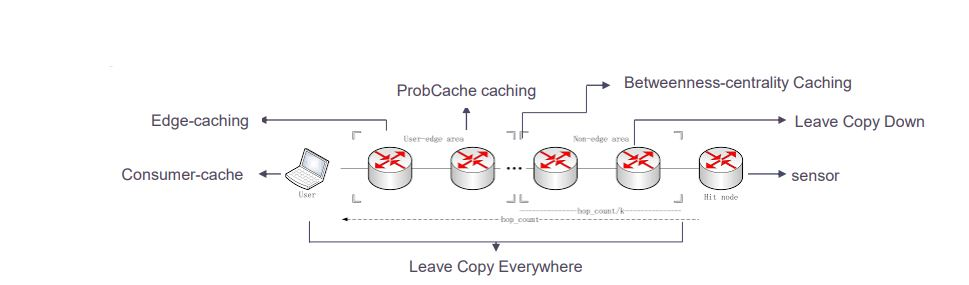
\includegraphics[width=13cm]{cachingStrategy}}
	\caption{استراتژی های متداول ذخیره‌سازی در شبکه‌های مبتنی بر محتوا برگرفته از\\ \lr{\href{https://mdpi-res.com/d_attachment/futureinternet/}{future internet}}}
	\label{fig:cachingStrategy}
\end{figure}

\subsection{سیاست جایگزینی محتوا}
در عمل به دلیل سایز محدود حافظه‌ی ذخیره‌سازی به یک سیاست مناسب برای جایگزینی محتوا در حافظه نیاز داریم. درواقع اصلی ترین هدف ما، یافتن بهینه ترین سیاست در تعامل با محیط می‌باشد به گونه‌ای که میزان تأخیر در ارسال دیتا برای یک محتوا را کمینه نماید.

  قطعاً استراتژی ذخیره‌سازی برای بعضی از محتویات که در طول زمان هیچ درخواستی برای آنها در شبکه وجود ندارد‌ و قبل از انتظار ما برای برآوردن درخواست دیتای مربوط به آنها منقضی می‌شود، مطلوب ما نیست. به عبارتی می توان گفت که در این حالت یک سیاست جایگزینی محتوای مناسب به کارایی استراتژی ذخیره‌‌سازی انتخاب شده، ‌کمک خواهد کرد. یک سری روش رایج جایگزینی برای شبکه‌های \lr{NDN} تعریف گردیده است که برجسته‌ترین و قدیمی‌ترین سیاست مطرح شده، \lr{FIFO (First Input, First Output)} می‌باشد.
  
  سیاست‌های جایگزینی مرسوم،‌ به چهار دسته مطابق با جدول\eqref{tab:replacementPolicies} تقسیم می‌گردند که در ادامه به آنها می‌پردازیم.
  \begin{table}[ht]
  	\caption{سیاست‌های مرسوم برای جایگزینی محتوا}
  	\label{tab:replacementPolicies}
  	\centering
  	\onehalfspacing
  	\begin{tabular}{|r|c|l|r|}
  		\hline \lr{Existing Plicies} & \lr{Description} & \lr{Category} \\ 
  		\hline \lr{LRU, LRU-threshold,} & \lr{Keeps the recently referenced objects} & \lr{Recency-based} \\
  			   \lr{LRU-hot, SLRU,} & \lr{} & \lr{} \\ 
  			   \lr{HLRU, LRU-LSC} & \lr{} & \lr{} \\ 
  		\hline \lr{LFU, LFU-Aging,} & \lr{Keeps the most requested objects} & \lr{Frequency-based} \\ 
  			\lr{LFU-DA, swLFU} & \lr{} & \lr{} \\
  		\hline \lr{RR, RAND,} & \lr{A simple random choice} & \lr{Randomized Policies} \\ 
  		\lr{HARMONIC} & \lr{to avoid computation overhead} & \lr{} \\
  		\hline \lr{SIZE, PSS, CSS} & \lr{Evicts large contents} & \lr{Size-based} \\ 
  		\hline 
  	\end{tabular} 
  \end{table}
  
  \subsubsection{\lr{Recency-Based Replacement Policies}}
  معروف‌‌ترین و پرکاربردترین سیاست از میان سیاست‌های جایگزینی محتوا در این دسته، سیاست \lr{LRU(Least Recently Used)} می‌باشد. (می توان گفت که سایر سیاست‌های متعلق به این دسته از سیاست \lr{LRU} مشتق شده‌اند.) در این حالت هریک از گره‌ها مجموعه‌ی درخواست‌های ارسال شده برای هریک از محتوا را دنبال می‌کند و زمانیکه نیاز به جایگزینی محتوا برای ذخیره‌ی محتوای جدید باشد، محتوایی را که اخیراً از آن کمتر از سایرین استفاده شده است را از حافظه دور می‌ریزد و فایل جدید را ذخیره می‌کند. روش مطرح شده نسبت به سایر سیاست‌های جایگزینی، کارایی بسیار بالایی دارد، اما در شرایطی که تعداد محتویات محبوب از سایز حافظه بیشتر باشد، شبکه دچار اختلال\footnote{\lr{thrashing}} خواهد شد.
  
  \subsubsection{\lr{Frequency-Based Replacement Policies}}
  سیاست اصلی در این گروه، سیاست \lr{LFU(Least Frequency Used)} می‌باشد. در واقع برخلاف سیاست \lr{LRU} که به سوال درباره‌ی آخرین بار استفاده از محتوا پاسخ می‌دهد،  سیاست \lr{LFU} میزان درخواست برای دیتای محتوا را دنبال می‌کند و در نهایت محتوا با کمترین میزان فرکانس درخواست را از حافظه حذف کرده و محتوای جدید را جایگزین آن می‌نماید و نسبت به سایر سیاست‌های جایگزینی، تنوع\footnote{\lr{diversity}} خوبی را برقرار می‌سازد اما بار بیشتری را در شبکه ایجاد می‌کند زیرا به جای آنکه فایل‌های محبوب‌تر را ذخیره نماییم، مجبور به ذخیره‌ی دیتای تازه هستیم یعنی به صورت مداوم برای واکشی پاسخ به حسگر مربوطه درخواست ارسال می‌نماییم که این امر باعث تخلیه‌ی باتری آن خواهد شد.
  
  \subsubsection{\lr{Randomized Replacement Policies}}
  این دسته از سیاست‌ها، سیاست‌های رندوم می‌باشند که در صورت تکمیل ظرفیت کش، از میان محتویات ذخیره شده یکی را به صورت رندوم انتخاب کرده و حذف می‌نماید و سپس محتوای جدید را جایگزین خواهد نمود. از این سیاست به عنوان معیاری\footnote{\lr{benchmark}} برای سنجش سایر سیاست‌ها استفاده می‌شود.
  
  \subsubsection{\lr{Size-Based Replacement Policies}}
  دامنه‌ی اصلی کاربرد این دسته از سیاست‌ها، ذخیره‌سازی محتوای وب می‌باشد که براساس سایز محتوا ذخیره‌سازی را انجام می‌دهد و سعی می‌شود که تا حدممکن محتوای با سایز کمتر را ذخیره نماید.
 
\subsection{متریک‌های مسئله}
برای مقایسه‌ی استراتژی‌های مختلف متریک‌های متعددی وجود دارد که غالباً شناخته شده نیز می‌باشند و شاید بتوان گفت که متریک‌هایی که در ادامه مطرح می‌شوند، کاملاً از یکدیگر مستقل نیستند. اولین متریک مطرح در یک مسئله‌ی ذخیره‌سازی بار سرور\footnote{\lr{server load}} و نسبت موفقیت حافظه‌ی کش در واکشی پاسخ\footnote{\lr{cache hit ratio}} می‌باشد. در شبکه‌های مبتنی بر محتوا منظور از موفقیت حافظه در واکشی پاسخ، زمانیست که مقدار دیتای مدنظرمان از روی مقادیر ذخیره شده در حافظه، واکشی شود. حال ضریب واکشی پاسخ از سرور زمانی رخ می‌دهد که دیتای مدنظرمان در حافظه‌ی کش ذخیره نشده باشد و مجبور باشیم تا مقدار آن را از گره تولیدکننده واکشی نماییم و بنابراین درخواست تا حسگر بالا رفته و اصطلاحاً بار سرور نیز افزایش می‌یابد. در واقع می توان گفت که دو پارامتر مطرح شده دوگان یکدیگر می‌باشند بدین معنا که با بالا رفتن میزان موفقیت حافظه‌ی کش در واکشی پاسخ، سرور مقدار بار کمتری را متحمل می‌شود.

\paragraph{}
متریک مطرح دیگر تأخیر بازیابی دیتا\footnote{\lr{data retrieval delay}} می‌باشد که به میانگین زمانی لازم برای واکشی دیتای مدنظرمان اطلاق می‌شود که باز ارسال‌های احتمالی را نیز شامل می‌گردد و بتبع این متریک می‌تواند تابعی از ازدحام\footnote{\lr{congestion}} در شبکه و یا تنوع در محتویات ذخیره شده باشد. هرچقدر که میزان تنوع در محتویات ذخیره شده بیشتر باشد، عملاً زمان کمتری برای واکشی پاسخ نیاز است. البته بالا بودن تنوع بیش از حدمجاز باعث می‌شود تا بی دلیل یک سری از محتویاتی را که به آنها نیازی نداریم، در حافظه ذخیره نماییم. درواقع برای اینکه بگوییم یک استراتژی ذخیره‌سازی تا چه میزان کارآمد می‌باشد، باید ببینیم که با چه سرعتی محتوای مدنظر را برایمان واکشی می نماید.  

\paragraph{}
متریک سوم نسبت بازارسال فایل‌های خواسته شده به دلیل اتمام مهلت\footnote{\lr{timed out}} آن به تمامی ارسال‌های موفق و ناموفق\footnote{\lr{interest retransmission ratio}} می‌باشد که عملاً مفهوم مستقلی از تأخیر و پارامتر قبلی نیست. درواقع همانطور که پیشتر نیز بدان اشاره شده، این متریک نیز تابعی از ازدحام و تنوع در محتویات ذخیره شده می‌باشد و علاوه براین به کارایی استراتژی ذخیره شده از سوی ما نیز بستگی دارد. در یک استراتژی ذخیره‌سازی ایده‌آل، تنوع تا حدمجاز بالا رفته و در ارسال های اولیه دیتای مدنظر از حافظه یا حسگر (بنا بر کارایی استراتژی به کار گرفته) واکشی می شود. درواقع این امکان وجود دارد که یک کپی از فایل مدنظرمان در گره‌های میانی ذخیره شده باشد و بتبع هرچه این گره به مصرف کننده نزدیکتر باشد، زمان کمتری برای بازارسال نیاز بوده و بتبع ترافیک کمتری نیز در شبکه خواهیم داشت. 

\paragraph{}
متریک چهارم میزان کل دیتای حذف شده از حافظه\footnote{\lr{total cache eviction}} می‌باشد که بیانگر سازگاری استراتژی انتخاب شده با میزان محبوبیت و پراکندگی توزیع آن در شبکه می‌باشد. حال هرچه‌قدر که استراتژی ذخیره‌سازی انتخاب شده موجب اختلال بیشتری در سیستم شود، میزان راندن محتویات از حافظه بالاتر می‌رود که نشان می‌دهد فایل‌های اولیه‌ی ذخیره شده در کش از محبوبیت کافی برخوردار نبوده یا حتی ممکنست این اتفاق به دلیل کم بودن حافظه‌ی اختصاص داده برای ذخیره‌سازی محتویات محبوب باشد. درواقع حذف یکسری از محتویات از حافظه گریزناپذیر می‌باشد ولی با اختصاص یک استراتژی مناسب می توان مقدار آن را متعادلتر نمود.

\paragraph{}
متریک تنوع در ذخیره‌سازی\footnote{\lr{cache diversity}}، بیانگر گوناگونی بین محتویات ذخیره شده می‌باشد و به صورت 
\begin{equation}\label{eq1}
	D = \frac{|C_{disj}|}{|S|}
\end{equation}
تعریف می‌گردد. مقدار \lr{S} تعداد کل محتویات تولید شده توسط گره تولیدکننده می‌باشد و هر گره تولیدکننده حداقل یک محتوا در جایی از شبکه دارد و مقدار 
\lr{$C_{disj}$} 
تعداد پیشوندهای متمایز برای تمامی مقادیر کش شده را مشخص می‌کند. این متریک تنوع در ذخیره‌سازی محتوا برای یک گره تولیدکننده را تا حد قابل قبولی تخمین می‌زند ولی در اینجا به دنبال متریکی برای بیان تنوع در سطح محتوا هستیم تا تعداد محتویات یکتا  و متمایز ذخیره شده را مشخص نماییم.

\paragraph{}
با توجه به توضیحات داده شده، برای مشخص کردن تنوع در سطح محتوا، متریک  نسبت نگهداری در حافظه\footnote{\lr{cache retention ratio}} معرفی می‌شود که متریک تنوع را تکمیل می‌نماید. درواقع این متریک نسبت محتویات متمایز ذخیره شده در کش را در یک لحظه‌ی خاص به کل محتویات متمایز در طول عمر شبکه نشان می‌دهد و با رابطه‌ی 
\begin{equation}\label{eq1}
	C = \frac{D_q}{D_p}
\end{equation}
به دست می‌آید. 

\section{استفاده از یادگیری تقویتی عمیق در تعیین سیاست جایگزینی محتوا}
حال مسئله‌ی اصلی ما ارائه‌ی روشی برای بهبود سیاست جایگزینی محتوا در حافظه‌ی کش می‌باشد که به ازای آن ترافیک شبکه و تأخیر پاسخدهی را متعادل‌تر نموده و میزان موفقیت استراتژی ذخیره‌سازی در واکشی دیتا را افزایش دهیم و درنتیجه‌ی آن مصرف انرژی در حسگرها نیز کاهش می‌یابد. با توجه به اینکه متدهای پیشنهادی براساس یادگیری ماشین قابلیت این امر را دارند که بسته به نیازهای محیط خود را به روز نمایند، به دنبال سیاستی مبتنی بر الگوریتمهای یادگیری ماشین هستیم تا بتواند تغییر توزیع محبوبیت فایل‌ها با زمان را مدیریت نماید. با توجه به غیرایستان\footnote{non-stationary} بودن محیط، سیاست جایگزینی محتوا مبتنی بر یادگیری تقویتی عمیق\footnote{\lr{deep reinforcement learning}} بدون هیچگونه فرضی مبنی بر رفتار کاربر، توزیع درخواست‌های ارسالی و یا حتی توزیع محبوبیت فایل‌ها می‌تواند چاره‌ساز باشد. 

به طور کلی یادگیری تقویتی متدی برای حل مسئله‌ی تصمیم‌گیری پی در پی برای محیط‌های غیرایستان است و در این فرآیند یادگیری عامل\footnote{\lr{agent}} که برای مسئله‌ی مطرح شده یک درگاه اینترنت اشیا می‌باشد با محیط تعامل داشته و اکشن‌هایی را اتخاذ می‌کند و بر محیط اثر می‌گذارد و از آن پاداش \footnote{\lr{reward}} دریافت می‌کند. این اکشن‌ها همان تصمیم‌گیری‌های جایگزینی محتوا در حافظه‌ی کش می‌باشد. در ابتدا عامل به صورت کاملاً رندوم برای شناخت محیط\footnote{\lr{exploration}}، اکشنی را انتخاب می‌کند و پس از آن براساس پاداش‌های دریافتی سعی می‌کند تا بیشترین بهره‌وری\footnote{\lr{exploitation}} از تعامل با محیط را به دست آورد.

تعاملات عامل با محیط به صورت یک فرآیند تصمیم‌گیری مارکوف\footnote{\lr{Markov Decision Process}} مدل می‌شود و تصمیم‌گیری در هر استیت براساس ارزش عمل در آن وضعیت انجام می‌شود. در واقع بیان ارزش استیت-اکشن و یا ارزش استیت به صورت صریح به دلیل پیوستگی فضای استیت‌ها،‌ غیر عملی می‌باشد و بنابراین با استفاده از  شبکه‌های عصبی عمیق تخمینی از آنها را به دست می‌آوریم. \cite{cachingtransientdata2018}

در اینجا با یک مسئله‌ی بهینه‌سازی سروکار داریم که قرار است تا در فواصل زمانی\footnote{\lr{time epoch}} آن مشخص نماییم که در صورت پر شدن گنچایش حافظه‌ی ذخیره‌سازی، محتوای جدید جایگزین کدام محتوا در حافظه شود و در این مدل باید تازگی داده را در نظر داشته باشیم و هدف اصلی مسئله، کمینه کردن تأخیر و مصرف انرژی حسگرها می‌باشد.

\subsection{مدل سیستم}
در عمل هرچقدر که حافظه‌ی ذخیره‌سازی به کاربران نزدیکتر باشد یا به عبارتی اگر عمل ذخیره‌سازی در نزدیکترین درگاه به گره‌های مصرف‌کننده یا لبه\footnote{\lr{edge node}} انجام گیرد، ترافیک شبکه متعادلتر می‌گردد زیرا برای واکشی پاسخ، دیگر درخواست تا گره تولیدکننده‌ی دیتا بالا نمی‌رود و در نتیجه تأخیر نیز بهبود می‌یابد. در واقع ذخیره‌سازی لبه، سریع‌ترین استراتژی برای واکشی پاسخ نسبت به سایر روش‌ها می‌باشد.

با این اوصاف، ساده‌ترین مدل متشکل از یک گره لبه می‌باشد که ماهیت فیزیکی آن می‌تواند به صورت یک ایستگاه پایه و یا درگاه شبکه‌های اینترنت اشیا تعریف شود. این گره تعدادی از مصرف‌کننده‌ها را پوشش می‌دهد. درواقع تمام درخواست‌های ارسالی در گره لبه جمع شده و بعد به سوی گره تولیدکننده‌ی دیتا پیش رانی می‌گردد. در مسیر عکس نیز دیتای تولید شده توسط گره یا گره‌های تولیدکننده در گره لبه جمع‌آوری شده و بعد برای کاربر فرستاده می‌شود.

گره‌های تولیدکننده‌ی دیتا می‌توانند حسگرها باشند که در ناحیه‌ی پوشش حداقل یک گره لبه قرار گرفته‌اند و داده‌هایی را با محتویات مختلف و مدت اعتبار محدود تولید می‌کنند و بدیهی است که هر تولیدکننده‌ی دیتا درخواست‌های متناسب با محتویات تولیدی خود را دریافت کند و به آنها پاسخ دهد.

\begin{figure}[ht]
	\centerline{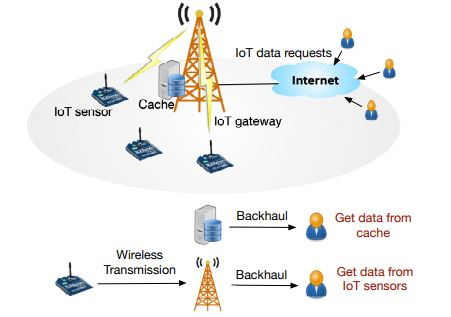
\includegraphics[width=8cm]{systemmodel}}
	\caption{نمایی از سیستم توصیف شده \cite{yao2020caching}}
	\label{fig:systemmodel}
\end{figure}

حال هرکدام از محتویات با یک شناسه‌ی یکتا\footnote{\lr{CID (Content Identifier)}} مشخص می‌گردد. در واقع در هریک از فایل‌ها، شناسه‌ی محتوا، دیتای مربوط به آن (مقدار اندازه گیری شده) به همراه دو برچسب زمانی که یکی بیانگر زمان تولید دیتا یا \lr{$t_{generation}$} و دیگری مدت زمان اعتبار مقدار اندازه‌گیری شده یا به تعبیر ریاضی \lr{$t_{life-time}$} می‌باشد. پارامتر طول عمر دیتا نیز به صورت 
\begin{equation}\label{eq3}
	T_{life} = t_{request} - t_{generation}
\end{equation}
 تعریف می‌شود که از مقایسه‌ی آن با مدت زمان اعتبار دیتا می توان به میزان تازگی دیتا پی برد.

همانطور که پیشتر گفته شد، در هریک از گره‌های لبه یک حافظه‌ی ذخیره‌سای قرار گرفته است. برای واکشی دیتای درخواست‌های ارسالی، در صورتیکه گره لبه محتوای درخواستی را ذخیره نکرده باشد، یک درخواست به گره تولیدکننده‌ی دیتا می‌فرستد و بعد دیتای موردنظر از گره تولیدکننده واکشی می‌شود. سپس گره لبه برای ذخیره یا عدم ذخیره‌ی دیتای به دست آمده یا اینکه آیا نیاز به جایگزینی محتوا در حافظه‌ی کش وجود دارد یا نه، تصمیم می‌گیرد و دیتا را برای کاربر می‌فرستد. حال اگر دیتای درخواست شده در حافظه‌ی کش وجود داشته باشد اما تازه نباشد یا به تعبیر ریاضی \lr{$t_{age} >= t_{life}$} باشد، آنگاه گره لبه برای آپدیت دیتا به گره تولیدکننده درخواست ارسال می‌نماید و پاسخ را برای گره مصرف‌کننده نیز می‌فرستد و مقدار قبلی دیتا را با مقدار جدید جایگزین می‌نماید. حال اگر دیتای درخواست شده در حافظه‌ی کش هنوز معتبر باشد یا به تعبیر ریاضی \lr{$t_{age} < t_{life}$} باشد، آنگاه گره لبه پاسخ را برای گره مصرف‌کننده می‌فرستد و بدین صورت از ارتباط مستقیم با حسگر برای واکشی جواب جلوگیری نمودیم و بنابراین مصرف انرژی حسگر کاهش یافته و حتی نیز با میزان تأخیر کمتری دیتای درخواستی برای گره مصرف‌کننده ارسال می‌گردد. سناریوی توصیف شده را در شکل \ref{fig:simplescenario} مشاهده می‌کنید.
\begin{figure}[ht]
	\centerline{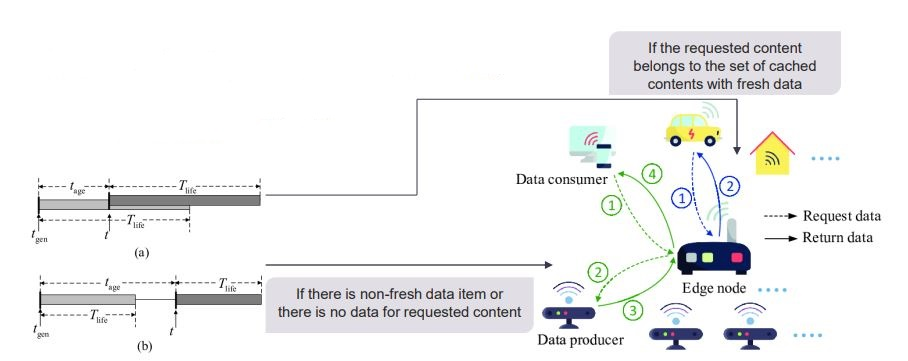
\includegraphics[width=15cm]{simplescenario}}
	\caption{سناریوی واکشی پاسخ در ذخیره‌سازی لبه برای شبکه‌های اینترنت اشیا\cite{cachingtransientdata2018}}
	\label{fig:simplescenario}
\end{figure}

\newpage
\subsection{آشنایی با نمادها و ادبیات یادگیری تقویتی به کار رفته در مسئله}
در این بخش توضیحاتی درباره‌ی نمادگذاری به کار رفته برای بیان ریاضی مسئله ارائه می‌گردد که این بیان در بین مقالات مرور شده در فصل دوم مشترک است.  مجموعه‌ی دیتای ذخیره شده در هر گره لبه در لحظه‌ی \lr{$t_k$} به صورت مجموعه‌ی 
\begin{equation}\label{eq4}
	D_k = \{d_k^1, d_k^2, ..., d_k^I\}
\end{equation}
 مشخص می‌شود. هر کدام از داده‌های ذخیره شده، گزارشی از مقدار یکی از محتویات موجود در شبکه می‌باشد که مجموعه‌ی این محتویات به صورت 
\begin{equation}\label{eq5}
	F_k = \{f_k^1, f_k^2, ..., f_k^I\}
\end{equation}
بیان می‌شود و تناظر یک به یک میان محتویات و دیتای اندازه گیری شده‌ی متناسب با هرکدام به کمک تابع 
\begin{equation}\label{eq6}
	d_k^i = p(f_k^i)
\end{equation}
 تعریف می‌گردد و مقدار \lr{I} برابر با حداکثر تعداد فایل‌هایی است که می‌توان در حافظه‌ی کش ذخیره‌سازی کرد. عامل در گره لبه برای تشخیص تازگی دیتای ذخیره شده نیز به صورت رابطه‌ی \ref{eq:7} عمل می‌نماید.
 \begin{equation}\label{eq:7}
 	d_k = \begin{cases}
 		p(f_k) \text{\lr{ if $f_k \in F_k, t_{age}(p(f_k)) < T_{life}(p(f_k))$}}\\
 		\text{\lr{new item, o.w.}}
 	\end{cases}
 \end{equation}

مفهوم تابع هزینه\footnote{\lr{cost function}} نیز برپایه‌ی هزینه‌ی از دست رفتن تازگی دیتای\footnote{\lr{freshness loss}} ذخیره شده و نیز هزینه‌ی ارتباط\footnote{\lr{communication loss}} برای واکشی پاسخ از حسگر یا حافظه‌ی اختصاص یافته در گره لبه درصورت موجود بودن دیتای درخواستی، مطابق رابطه‌ی\ref{eq:8} تعریف می‌شود. در اینجا \lr{$c_2 > c_1$} است.
\begin{equation}\label{eq:8}
	c(d_k) = \begin{cases}
		c_1 \text{\lr{ if $f_k \in F_k, t_{age}(p(f_k)) < T_{life}(p(f_k))$}}\\
		c_2 \text{\lr{ o.w.}}
	\end{cases}
\end{equation}  
 
 تابع هزینه‌ی مربوط به از دست رفتن اعتبار دیتا به صورت رابطه‌ی\ref{eq:9} تعریف می‌شود که تنها در حالتی که دیتای درخواستی در حافظه موجود و معتبر یاشد، مقدار دارد زیرا که در سایر حالات دیتای معتبر از گره تولیدکننده‌ی مربوطه واکشی می‌گردد و در نتیجه مدت زیادی از زمان تولید آن نگذشته است. 
 \begin{equation}\label{eq:9}
 	l(d_k) = \begin{cases}
 		\frac{t_{age}(p(f_k))}{T_{life}(p(f_k))} \text{\lr{ if $f_k \in F_k, t_{age}(p(f_k)) < T_{life}(p(f_k))$}}\\
 		0 \text{\lr{ o.w.}}
 	\end{cases}
 \end{equation}  
  در نهایت نیز تابع هزینه به صورت میانگین وزن‌دار هزینه‌ی ارتباط و هزینه ی از دست رفتن اعتبار دیتا تعریف می‌شود:
  \begin{equation}\label{eq:10}
  	C(d_k) = \alpha . c(d_k) + (1 - \alpha) . l(d_k)
  \end{equation}

و تابع سودمندی\footnote{\lr{utility function}}، مفهومی در برابر تابع هزینه بوده و به صورت نمایش داده شده در رابطه‌ی\ref{eq:11} مشخص می‌گردد.
\begin{equation}\label{eq:11}
	U(d_k) = B - C(d_k)
\end{equation}

در رابطه‌ی \ref{eq:11} معمولاً مقدار \lr{B} به صورتی تعریف می‌شود که تابع سودمندی به صورت نمایش داده شده در آید:
\begin{equation}\label{eq:12}
	U(d_k) = \alpha . (c_2 - c(d_k)) + (1 - \alpha) . g(d_k)
\end{equation}

در رابطه‌ی \ref{eq:12} منظور از تابع \lr{g(d)} تازگی دیتاست، که به صورت 
\begin{equation}\label{eq:13}
	g(d) = \frac{T_{life}(p(f_k)) - t_{age}(p(f_k))}{T_{life}(p(f_k))} 
\end{equation}  
تعریف می‌شود.

فضای حالات برای جایگزینی محتوا در حافظه براساس محتویات داخل حافظه، دیتای مربوط به هریک از آنها و نیز میزان تازگی یا اعتبار دیتای ذخیره شده، تعیین می‌شود. (این مقادیر حداقل اطلاعات مورد نیاز برای تعیین حالت عامل است. در حالتی که گره‌ها متحرک هستند برای تعیین حالت اطلاعات بیشتری مورد نیاز خواهد بود که در مقالات فصل دوم درباره‌ی آنها بیشتر بحث می‌شود.) با توجه به اینکه میزان اعتبار دیتا به صورت رابطه‌ی \ref{eq:13} به دست می‌آید می توان گفت که فضای حالات در مسئله‌ی ما پیوسته است. 

به طور کلی در صورتی که از گنجایش حافظه‌ی ذخیره‌سازی باقی مانده باشد هر فایل درخواستی که از حسگر واکشی می‌شود در آن ذخیره می‌گردد. حال اگر حافظه‌ی ذخیره‌سازی پر شود، فایل با محبوبیت کمتر از حافظه حذف شده و جای خود را به فایل جدید می‌دهد. حال اگر فایل درخواستی در حافظه موجود باشد ولی اعتبار خود را از دست داده باشد دوباره نیاز داریم تا داده‌ی معتبر را از گره تولیدکنده ی مربوطه واکشی نماییم و دیتای مربوط به آن به روز رسانی می‌شود. اکشن‌های توصیف شده در حالات مختلف فضای اکشن‌ها را برای ما مشخص می‌نماید و اینکه در شرایط مختلف چه عملی بهینه تلقی می‌گردد، سیاست بهینه را برای ما مشخص می‌سازد. حال محیط پاداشی را پس از اعمال اکشن اتخاذ شده به عامل می‌دهد و حال اینکه توزیع پاداش به چه صورت باید باشد یا به عبارتی چگونگی شبیه‌سازی آن در مسئله‌ سوال مهمی است که پیاده‌سازی متفاوتی برای آن در مقالات انجام شده است. 
 
 حال در  مقالاتی که در فصل دوم ارائه می‌گردد، تفاوت در الگوریتم‌های به کار رفته برای تخمین ارزش استیت‌ها ارزش استیت-اکشن‌ها یا حتی سیاست بهینه می‌باشد. در بعضی نیز بنا به شرایط محیطی، پارامترهایی برای تعیین استیت به مسئله اضافه می‌شود یا در برخی دیگر از الگوریتم‌های یادگیری عمیق سلسله مراتبی\footnote{\lr{Hierarchical Deep Reinforcement Learning}} برای تعیین سیاست جایگزینی محتوا در حافظه استفاده می‌شود که این به معنی استفاده از یک استراتژی جدید مبنی بر قرار دادن حافظه‌ی ذخیره‌سازی در گره‌های لبه و یک لایه دورتر از گره‌های مصرف‌کننده (اصطلاحاً معماری ریشه-برگ\footnote{\lr{parent-leaf architecture}}) می‌باشد.

\section{جمع بندی}
به طور کلی دو ویژگی منحصربفرد شبکه‌های اینترنت اشیا یکی محدودیت سطح انرژی حسگرها و دیگری محدودیت مدت زمان اعتبار دیتا، مسئله‌ی ذخیره‌سازی در این شبکه‌ها را در مقایسه با استراتژی ذخیره‌سازی در سایر شبکه های مبتنی بر محتوا متمایز می‌سازد. علاوه براین با توجه به غیرایستان بودن محبوبیت فایل‌ها در طول زمان، به کارگیری یک استراتژی مبتنی بر یادگیری تقویتی عمیق برای جایگزینی محتوا در حافظه‌ی ذخیره‌سازی با توجه به محدودیت گنجایش آن، می‌تواند زمان لازم برای واکشی پاسخ را کاهش داده و نیز ترافیک شبکه را متوازن‌تر نماید و در نتیجه‌ی آن مصرف انرژی حسگر یا گره تولیدکننده‌ی داده کاهش می‌یابد. فصل دوم نیز به مرور مقالات مطالعه شده اختصاص یافته است.





		% فصل اول: مقدمه
% !TeX root=../main.tex
\chapter{مروری بر مطالعات انجام شده}
%\thispagestyle{empty} 
\section{مقدمه}
در این فصل به مرور تعدادی از مقالات مربوط به استراتژی ذخیره‌سازی و سیاست جایگزینی محتوا در حافظه برای شبکه‌های اینترنت اشیا می‌پردازیم. در ادامه الگوریتم‌های استفاده شده در مقالات، معماری به کار رفته برای پیاده‌سازی و چالش‌های آن برای محیط  استفاده شده به طور اجمالی بیان می‌شوند. 

\section{مروری بر ادبیات موضوع}

\subsection{\lr{Deep Reinforcement Learning for Cooperative Content Caching in Vehicular Edge Computing and Networks}}
با توجه به ماهیت محیط و حرکت گره‌های مصرف کننده،‌در مقاله‌ی \cite{qiao2019deep} تعریف حالت با آنچه که پیشتر دیدیم تفاوت‌هایی دارد، در ضمن فضای اعمال مجاز نیز دیگر گسسته نخواهد بود که بتبع این مسئله پیچیدگی‌های بسیاری را به وجود می آورد. در ابتدا درباره‌ی فضای استیت‌ها و اکشن‌ها توضیحاتی داده می‌شود:

\paragraph{فضای استیت‌ها}
در ابتدای هر بازه‌ی زمانی، عامل هوشمند به اطلاعاتی درباره‌ی محتوای درخواستی توسط وسایل نقلیه\footnote{\lr{content requesting vehicles(CRV)}} دست پیدا می‌کند که این اطلاعات حالت عامل در این بازه‌ی زمانی را برای ما مشخص می‌کند و این مؤلفه‌ها عبارتند از:  
\begin{itemize}
	\item 
	نوع محتوای درخواست شده در بازه‌ی زمانی ذخیره‌سازی 
	\item 
	مهلت تحویل دیتای درخواستی در بازه‌ی زمانی ذخیره‌سازی کنونی
	\item
	سایز باقیمانده از دیتای درخواستی برای ارسال در بازه‌ی زمانی کنونی
	\item
	مؤلفه‌ی مربوط به منطقه‌ای که دیتای مربوط به محتوای درخواستی موجود بوده یا مؤلفه‌ی مربوط به موقعیتی که دیتای درخواستی ذخیره شده است.
	\item 
	میزان محبوبیت محتوای درخواستی در بازه‌ی زمانی فعلی
	\item 
	بیانگر عملیات ذخیره‌سازی\footnote{\lr{caching indicator}} که نشان می‌دهد در بازه‌ی زمانی ذخیره‌سازی فعلی، ذخیره‌ی دیتای درخواستی در کدام گره ذخیره‌سازی انجام شود.
\end{itemize}

\paragraph{فضای اکشن‌ها}
بعد از دریافت درخواست محتوا، رسانه‌ی همه‌پخشی ماهواره‌ای\footnote{\lr{Media Broadcast Satellite(MBS)}} محبوبیت محتوای درخواست شده را محاسبه می‌کند و از روی آن تصمیم می‌گیرد که‌ آیا لازم است دیتای مربوط به محتوای درخواستی ذخبره شود یا خیر و در صورتیکه پاسخ مثبت باشد،‌ گره مناسب برای ذخیره‌ی دیتا را مشخص می‌نماید. در هر بازه‌ی زمانی مربوط به واکشی پاسخ، مقادیر زمان‌بندی برای هریک از وسایل و نیز پهنای باند تخصیص یافته به هرکدام، توأماً برای کاهش هزینه‌ی دسترسی به محتوا با قید مهلت مربوط به ارسال پاسخ مورد استفاده قرار می‌گیرند. بنابراین فضای اکشن‌ها با مؤلفه‌هایی که در ادامه توصیف می‌شوند، مشخص می‌گردد.
\begin{itemize}
	\item 
	آیا محتوای درخواستی در بازه‌ی زمانی ذخیره‌سازی در حافظه وجود داشته است یا خیر. در صورتیکه جواب مثبت باشد، مقدار این مؤلفه 1 خواهد بود.  
	\item 
	نشانگر ارتباط\footnote{\lr{association indicator}} بین محتوای درخواستی و گره لبه، در واقع این مولفه مشخص می‌کند تا برای واکشی پاسخ باید به سراغ کدامیک از گره‌های لبه برویم.
	\item
	پهنای باندی که به ازای آن ارتباط بین گره لبه و وسیله‌ی درخواست دهنده برقرار می‌شود.
\end{itemize}
 
 در اینجا با توجه به پیوسته بودن فضای استیت‌ها و به طور ویژه اکشن‌ها به جای تخمین ارزش استیت ها یا ارزش استیت‌-اکشن‌ها (که به کمک شبکه یا شبکه‌ها‌ی عصبی صورت می‌پذیرد) ، به طور مستقیم سیاست بهینه را با استفاده از الگوریتم \lr{Deep Deterministic Policy Gradient}(\ref{fig:DDPG}) تخمین می‌زنیم.
 \begin{figure}[ht]
 	\centerline{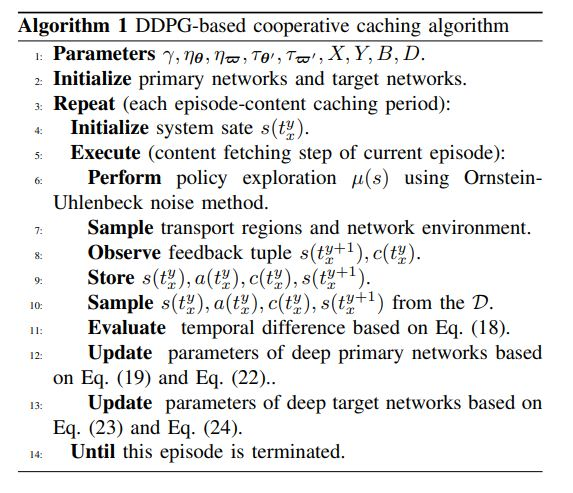
\includegraphics[width=11cm]{DDPG}}
 	\caption{الگوریتم \lr{Deep Deterministic Policy Gradient}}
 	\label{fig:DDPG}
 \end{figure}

الگوریتم پیشنهادی مقاله در زمره‌ی یادگیری بدون مدل\footnote{\lr{Model-free Learning}} به‌ شمار می‌رود که براساس تعداد بسیاری از تجربیات و تعاملات با محیط، تخمین سیاست صورت می‌پذیرد. برای بیان چرایی و مزیت این الگوریتم نسبت به سایر الگوریتم‌های مشابه، در ادامه توضیحاتی درباره‌ی سه مدل مختلف یادگیری بدون مدل ارائه می‌گردد. 

\begin{itemize}
	\item \textbf{مدل مبتنی بر ارزش\footnote{\lr{value-based approach}} یا مدل نقاد\footnote{\lr{critic model}}}\\
	در این روش، سیاست بهینه براساس مقادیر مربوط به تخمین ارزش استیت-اکشن‌ها \lr{$Q(s, a)$} به دست می‌آید. 
	\item \textbf{مدل مبتنی بر سیاست\footnote{\lr{policy-based approach}} یا مدل عملگر\footnote{\lr{actor model}}}\\
	این روش می‌تواند سیاست مبتنی بر احتمالات (احتمال قرار گرفتن در یک استیت مشخص با توجه به غیرایستان بودن محیط) \lr{$\pi_{\overline{\omega}}(s|a)$} را یاد بگیرد.
	
	\item \textbf{روش عملگر-نقاد\footnote{\lr{actor-critic}}}\\
	این روش ترکیبی از دو روش قبلی می‌باشد که در این مقاله به کمک الگوریتم \lr{policy gradient} در عملگر، سیاست بهینه تخمین زده می‌شود و براساس فیدبکی که نقاد برای ارزش استیت-اکشن‌ها تولید می‌کند، سیاست مذکور اصلاح می گردد. درواقع این دست از الگوریتم‌ها برای هر دو فضای اکشن‌های پیوسته و گسسته مناسب می‌باشند که نمونه‌ی گسسته‌ی آن را در ادامه می‌بینیم. البته همگرایی و کارآمدی الگوریتم‌های عملگر-نقاد به تعداد نمونه‌ها و تعاملات با محیط وابسته است.
	
\end{itemize}

\begin{figure}[ht]
	\centerline{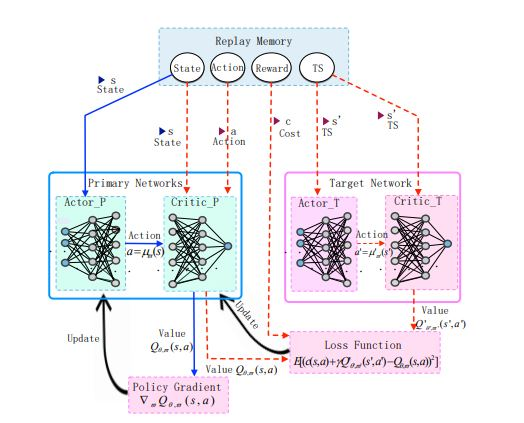
\includegraphics[width=10cm]{PG}}
	\caption{دیاگرام \lr{Deep Deterministic Policy Gradient}}
	\label{fig:PG}
\end{figure}

 همانطوری که در شکل \ref{fig:PG} مشاهده می‌شود، این مقاله از شبکه‌های عصبی عمیق برای تخمین دقیق تابع قطعیت سیاست\lr{$\mu(s)$} و ارزش استیت-اکشن‌هاlr{$Q(s, a)$} استفاده می‌کند. همانطوری که می‌بینید فریمورک به کار رفته از سه ماژول اصلی تشکیل می‌شود: شبکه‌های مقدماتی\footnote{\lr{primary networks}}، هدف\footnote{\lr{target networks}} ( که در هریک شبکه‌های عمیق عملگر\footnote{\lr{deep actor-network}} و نقاد\footnote{\lr{deep critic-network}} نقش اصلی را ایفا می‌کنند) و حافظه‌ی بازپخشی\footnote{\lr{replay memory}}.

\subsection{\lr{Caching Transient Content for IoT Sensing: Multi-Agent Soft Actor-Critic}}
در مقاله‌ی \cite{wu2021caching} برای اولین بار راه حلی برای مسئله‌ی به روز رسانی حافظه‌ی کش برای یک محیط چندعامله و متشکل از چندین گره لبه ارائه شده و این مسئله به صورت یک فرآیند تصمیم‌گیری مارکوف مشارکتی بین چندعامل براساس کاهش مقدار تابع وزنداری از طول عمر آیتم هر محتوا، هزینه‌ی به روزرسانی حافظه‌ی ذخیره‌سازی، بارترافیکی شبکه و کاهش مصرف انرژی در واکشی پاسخ مطرح گردیده است. 

در اینجا یک نسخه از الگوریتم چندعامله‌ی \lr{Soft Actor-Critic} با فضای اعمال گسسته ایجاد شده است که تعداد عامل‌های الگوریتم خروجی به طور خطی با تعداد گره‌های لبه و حسگرهای شبکه‌های اینترنت اشیا قابل افزایش است. برای رسیدن به این هدف، در این مقاله از یک \lr{Gumble-SoftMax-sampler} برای نمونه‌برداری از محیط استفاده شده است که پارامترهای مربوط به آن را برای رسیدن به فضای اعمال دیفرانسیل‌پذیر تنظیم می‌نماید. در آخر نیز برای برقرای توازن میان اکتشاف و بهره‌وری (که مسئله‌ی مشترک میان تمامی الگوریتم‌های یادگیری تقویتی می‌باشد) از یک تنظیم‌ساز آنتروپی\footnote{\lr{Entropy Regularization}} برای جلوگیری از همگرایی زودهنگام استفاده می‌شود.

برای کاهش سربار ارتباط میان گره‌های لبه و لایه‌ی ابری، هریک از الگوریتم‌های \lr{Soft Actor-Critic} و \lr{Deep Q-Network} در دو حالت روش کنترلی متمرکز و غیرمتمرکز پیاده‌سازی و مقایسه شده‌اند. در سیاست کنترلی غیرمتمرکز\ref{fig:decentralized}، هرکدام از سرورهای گره‌های لبه به عنوان یک عامل مستقل، براساس مشاهدات خود تصمیماتی را برای ذخیره‌کردن، جایگزینی محتوا و ... اتخاذ می‌نماید اما در روش کنترلی متمرکز\ref{fig:centralized} از یک پردازنده‌ی ابری\footnote{\lr{Cloud Processor}} برای بهبود پاداش‌های دریافتی سیستم و بالا بردن هماهنگی با سایر گره‌های لبه استفاده می‌شود.

\begin{figure}[ht]
	\centering 
	\subfloat[روش کنترلی متمرکز]{ \label{fig:centralized}
		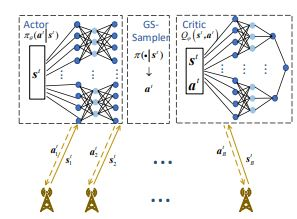
\includegraphics[width=0.4\textwidth]{centralized}}
	\hspace{10mm}
	\subfloat[روش کنترلی غیرمتمرکز]{ \label{fig:decentralized}
		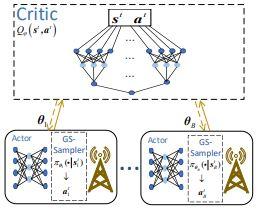
\includegraphics[width=0.4\textwidth]{decntralized}}%
	\caption{دیاگرام الگوریتم \lr{SAC} به کاررفته}
	\label{fig:centralizedvsdec} %% label for entire figure
\end{figure}
\pagebreak

همانطوری که در شکل \ref{fig:centralizedvsdec} دیده می‌شود، در الگوریتم متمرکز، پردازنده‌ی ابری نقش یک عامل متمرکز را ایفا می‌کند و سیاست متمرکز برای تمامی گره‌های لبه را یاد می‌گیرد. متناسباً هریک از گره‌های لبه ابتدا مشاهدات خود را در هر واحد زمانی برای پردازنده‌ی ابری می‌فرستند و سپس پس از آنکه پردازنده‌ی ابری مشاهدات محلی آنها را جمع‌آوری کرد، عملکرد بهینه برای هریک از گره‌های لبه را ارسال می‌نماید. 

در آخر نیز، عملکرد الگوریتم \lr{SAC} در حالت متمرکز و غیر متمرکز با روش‌های عملگر-نقاد معمول و روش \lr{DQN} مقایسه شده است. به طور کلی، متوسط پاداش دریافتی برای \lr{Decentralized SAC} نسبت به \lr{Centralized SAC} بیشتر بوده و مقدار به دست آمده حاصل از الگوریتم \lr{Centralized SAC} از الگوریتم عملگر-نقاد معمول بیشتر بوده و برای الگوریتم عملگر-نقاد معمول نسبت به \lr{DQN} بیشتر است و البته باید به این نکته اشاره کرد که متوسط پاداش به دست آمده برای الگوریتم \lr{DQN} نسبت به سایر الگوریتمها نویزی‌تر نیز می‌باشد. 


%\begin{figure}[ht]
%	\centerline{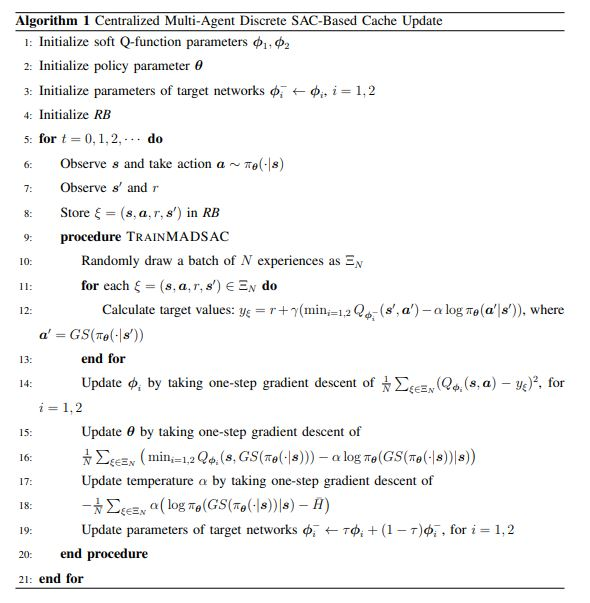
\includegraphics[width=8cm]{centralizedSAC}}
%	\caption{الگوریتم \lr{Centralized Soft Actor-Critic}}
%	\label{fig:cSACAlgo}
%\end{figure}

%\begin{figure}[ht]
%	\centerline{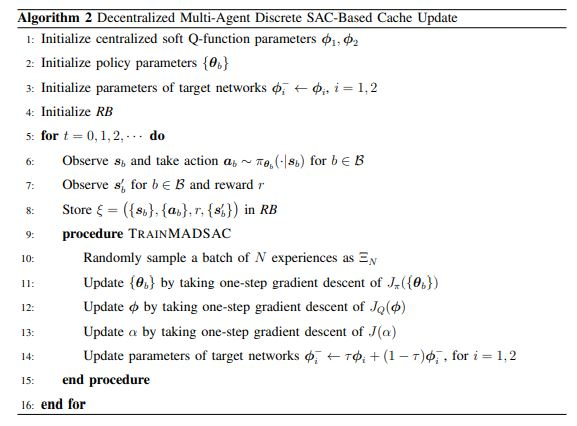
\includegraphics[width=8cm]{decentralizedSAC}}
%	\caption{الگوریتم \lr{Decentralized Soft Actor-Critic}}
%	\label{fig:dSACAlgo}
%\end{figure}

\subsection{\lr{A Deep Reinforcement Learning-Based Caching Strategy for IoT Networks with Transient Data}}

مقاله‌ی \cite{wu2022deep} از وجود لایه‌های مختلف در معماری شبکه‌های اینترنت اشیا بهره می‌برد و مدلی متشکل از دو لایه با یک گره پدر\footnote{\lr{parent node}} در لایه‌ی بالایی و چندین گره برگ\footnote{\lr{leaf}} یا لبه در لایه‌ی پایین‌تر شبکه در نظر می‌گیرد و تمامی این گره‌ها از قابلیت ذخیره‌سازی برخوردارند. شکل \ref{fig:parent-leaf} معماری در نظر گرفته شده در این مقاله را نشان می‌دهد.

\begin{figure}[ht]
	\centerline{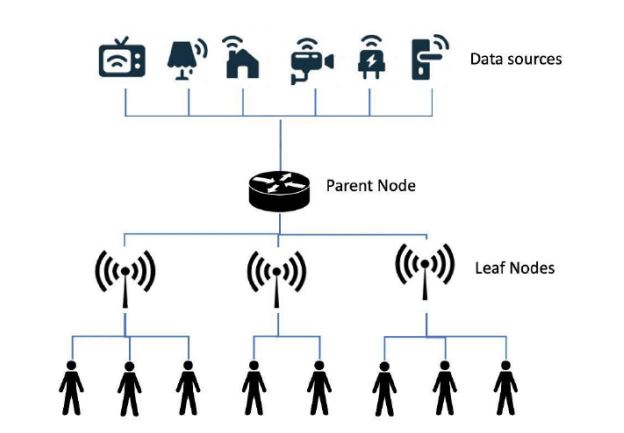
\includegraphics[width=10cm]{parent-leaf}}
	\caption{نمایی از معماری ریشه-برگ}
	\label{fig:parent-leaf}
\end{figure}

بنابراین می‌توان گفت که شبکه‌های اینترنت اشیا موجودیت‌های مختلفی از جمله افزاره‌های شبکه‌های اینترنت اشیا، گره ریشه، گره‌های برگ یا لبه و کاربران را شامل می‌شوند. 

\begin{itemize}
	\item \textbf{افزاره‌های شبکه‌های اینترنت اشیا}\\
	این افزاره‌ها در دنیای فیزیکی تعبیه می‌شوند و از آنها انتظار می‌رود تا پارامتری در محیط را اندازه‌گیری کرده و گزارش دهند یا بخشی از محیط را کنترل نمایند. گاهی نیز ممکنست اعتبار داده‌ی گزارش شده توسط آنها به حدی کم باشد که عملاً فایل تولید شده قابل ذخیره‌سازی نباشد.
	\item \textbf{گره ریشه}\\
	این نوع از گره‌ها لایه‌های درونی شبکه را شکل می‌دهند و مانند درگاهی که از یک طرف تمامی افزازه‌های شبکه‌ی اینترنت اشیا به تمامی گره‌های لبه یا برگ از طرف دیگر متصل می‌کند، عمل می‌نماید. درواقع این گره درخواست را از طرف گره‌های لبه دریافت می‌کند و پاسخ را از افزاره‌های مربوطه واکشی کرده و سپس برای گره‌های لبه می‌فرستد.
	\item \textbf{گره برگ}\\
	این دسته از گره‌ها نزدیکترین درگاه به کاربران هستند و میزان پوشش آنها به صورت منطقه‌ای و در حد تعدادی از کاربران می‌باشد، این گره‌ها به گره ریشه متصل هستند. 
	\item \textbf{کاربران}\\
	درواقع منظور از کاربران می‌تواند اپلیکیشن‌هایی برای پایش دیتای تولیدشده توسط حسگرها باشد. در این مقاله فرض شده است که حرکت کاربران محدود بوده و اتصال بین کاربر و گره برگ پایدار است در واقع این بدین معنیست که کاربر از دامنه‌ی پوشش گره برگ قبل از رسیدن پاسخ خارج نمی‌شود. 
\end{itemize}

این مقاله برای مشخص کردن رتبه‌بندی فابل‌ها به لحاظ محبوبیت در استراتژی ذخیره‌سازی و جایگزینی محتوا از الگوریتم \lr{Proximal Policy Optimization} (\ref{fig:ppo}) به سبک عملگر-نقاد در دو حالت متمرکز و غیرمتمرکز استفاده می‌کند. در حالت متمرکز هریک از گره‌های برگ تصمیمات مربوط به ذخیره‌سازی یا جایگزینی محتوا در حافظه را می‌گیرد اما در حالت غیرمتمرکز گره ریشه بر روی تصمیمات ذخیره‌سازی اثر می‌گذارد و محتویات 
ذخیره‌سازی در هریک از گره‌های برگ را مشخص می‌کند و محتویات مشترک میان آنها در گره ریشه ذخیره می‌گردد.

\begin{figure}[ht]
	\centerline{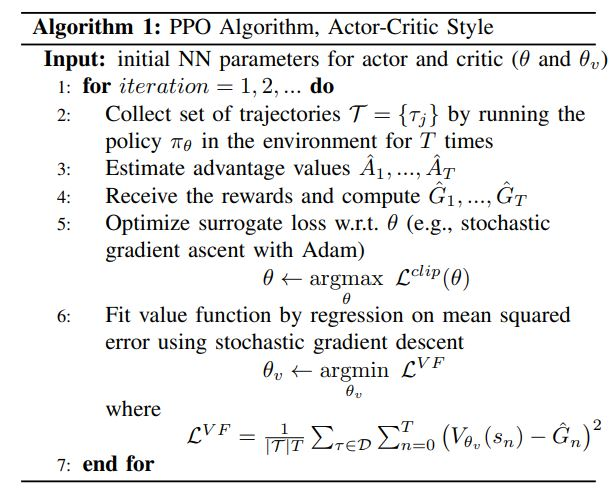
\includegraphics[width=11cm]{PPO}}
	\caption{الگوریتم \lr{Proximal Policy Optimization}}
	\label{fig:ppo}
\end{figure}

همانطوری که در شکل \ref{fig:ppo} می‌بینید در اینجا نیز از یک سیاست پارامترایز شده \lr{$\pi_{\theta}(a|s)$} برای تخمین محبوبیت فایل‌ها در محیط غیرایستان استفاده می‌شود که برای محیط‌های چندعامله نیز قابل پیاده‌سازی است و به این دلیل این الگوریتم نیز در گروه الگوریتم‌های \lr{policy gradient} قرار می‌گیرد. در اینجا نیز دو شبکه‌ی عصبی عملگر برای تخمین سیاست و نقاد برای تخمین ارزش استیت‌ها \lr{$V^{\pi_{\theta}}(s; \theta_{\nu})$} به کار رفته‌اند. علاوه بر حل مسئله‌ی بهینه‌سازی برای یافتن سیاست بهینه، یکی از اهداف الگوریتم بهینه‌سازی تابع \lr{clipped Surrogate} که از \lr{stochastic gradient ascent} استفاده می‌کند، می‌باشد. در واقع از این تابع برای آپدیت پارامتر سیاست بهینه با پارامتر \lr{$\theta$} توسط شبکه‌ی عملگر براساس فیدبک نقاد طبق مشاهدات در تعامل با محیط استفاده می‌شود. تابع هدف \lr{clipped Surrogate} به صورت 
\begin{equation}\label{eq:20}
	\mathcal{L}^{clip}(\theta) = E_{\pi}[\min(b_n(\theta)A_n, clip(b_n(\theta), 1 - \epsilon, 1 + \epsilon)A_n)]
\end{equation}  
\begin{equation}\label{eq:21}
	b_n(\theta) = \frac{\pi_{\theta}(a_n|s_n)}{\pi_{\theta_{old}}(a_n|s_n)}
\end{equation}  
تعریف می‌شود.

درواقع تابع \lr{$clip$} یک نسبت احتمالاتی \lr{$b_n(\theta)$} را که مطابق با رابطه‌ی \ref{eq:21} تعریف می‌شود، از ورودی می‌گیرد که اگر مقدار آن از \lr{$1-\epsilon$} کمتر و یا از \lr{$1+\epsilon$} بیشتر نباشد، همان را به عنوان خروجی برمی‌گرداند و در غیر اینصورت یکی از این مقادیر را جایگزین می‌نماید. همانطوری که می‌دانید \lr{$\theta_{old}$} مقدار پیشین این پارامتر قبل از آپدیت می‌باشد و مقدار \lr{$A_n$} به صورت
\begin{equation}\label{eq:20}
	A_n = r_n +‌\gamma V^{\pi_{\theta}}(s_{n+1}) - V^{\pi_{\theta}}(s)
\end{equation}  
تعریف می‌شود و مقداار \lr{$\theta$} به صورت
\begin{equation}\label{eq:20}
	\theta \leftarrow \arg\max \mathcal{L}^{clip}(\theta)
\end{equation}
آپدیت می‌شود.

در نهایت نیز همانطوری که مورد انتظار است، متوسط مجموع پاداش‌های دریافتی در حالت غیرمتمرکز (در حالیکه فرمان ذخیره یا جایگزینی محتوا از سوی گره ریشه به گره های برگ صادر می‌شود) نسبت به حالت متمرکز به مقدار بیشتری همگرا می‌شود و با به کار گرفتن روش کنترلی غیرمتمرکز در محیط ذکر شده در مقاله، مقدار تأخیر و ترافیک در شبکه متوازن‌تر می‌شود.
\pagebreak
در شکل \ref{fig:ppod} دیاگرام مربوط به الگوریتم \lr{Proximal Policy Optimization} در مقاله‌ی \cite{wu2022deep} آورده شده است.

\begin{figure}[ht]
	\centerline{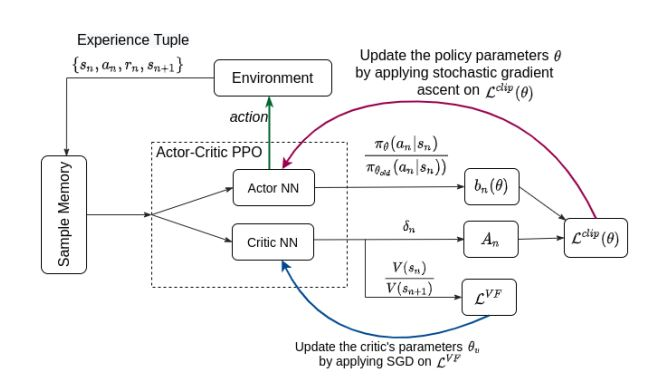
\includegraphics[width=14cm]{PPO-diagram}}
	\caption{دیاگرام \lr{Proximal Policy Optimization}}
	\label{fig:ppod}
\end{figure}

\newpage
\subsection{\lr{HFDRL: An Intelligent Dynamic Cooperate Cashing Method Based on Hierarchical Federated Deep Reinforcement Learning in Edge-Enabled IoT}}

در الگوریتم یادگیری تقویتی عمیق فدراسیونی سلسله مراتبی\footnote{\lr{Hierarchical Federated Deep Reinforcement Learning}} پیشنهادی مقاله‌ی \cite{majidi2021hfdrl}، ابتدا به صورت سلسله مراتبی گره‌های لبه با استفاده از الگوریتم \lr{Fuzzy C-Means} طبقه‌بندی می‌شوند. اساس طبقه‌بندی پارامترهایی مانند موقعیت جغرافیایی، ویژگی‌های مربوط به کاربران (از قبیل سن، جنسیت و ...) و خصوصیات درخواست‌های ارسالی (از قبیل نوع،‌ دیتاسنتر مربوطه و ...)، می‌باشد که ماهیت غیرایستان بودن محیط نیز در خوشه‌بندی در نظز گرفته شدا است زیرا در طول زمان الگوی درخواست‌های ارسالی کاربران تغییر می‌کند. همانطوری که در شکل \ref{fig:cluster-levels} دیده می‌شود، خوشه‌های در طبقه‌بندی اول با کمترین میزان تأخیر می‌توانند ارتباط را برقرار کنند و بیشترین مبادله‌ی محتویات را داشته باشند. در سطح بعدی هرکدام از خوشه‌ها به منزله‌ی یک گره تلقی می‌گردند و خوشه‌بندی در لایه‌ی بعدی نیز عیناً طبق پارامترهای مورد استفاده در خوشه‌بندی لایه‌ی قبلی، انجام می‌پذیرد. در صورت نیاز به لایه‌های بیشتر، خوشه‌بندی در آنها به همین منوال صورت می‌گیرد. 

\begin{figure}[ht]
	\centerline{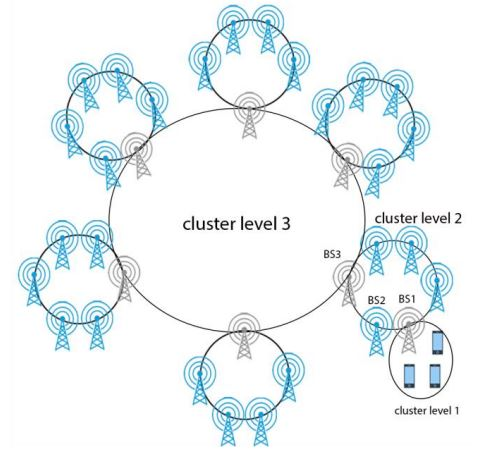
\includegraphics[width=10cm]{cluster-levels}}
	\caption{خوشه‌بندی سه‌لایه‌ای از ایستگاه‌های پایه}
	\label{fig:cluster-levels}
\end{figure}

در یادگیری تقویتی عمیق سلسله‌مراتبی و فدراسیونی هر کدام از گره‌های لبه در شبکه تابع ارزش استیت-اکشن‌ها را به کمک یک شبکه‌ی یادگیری تقویتی عمیق تخمین می‌زند و مقدار محبوبیت فایل‌ها زا نیز پیش‌بینی می‌کند و براساس آن دیتا را ذخیره کرده و یا آن را از حافظه حذف می‌نماید.  

پس از خوشه‌بندی هریک از گره‌های لبه،‌ هرگاه که درخواستی به ایستگاه پایه ارسال می‌شود ابتدا لازم است تا مشخص شود که آیا محتوای درخواست شده قبلاً ذخیره شده است یا خیر که در صورت مثبت بودن پاسخ باید ایستگا‌هی که دیتا در آن ذخیره شده مشخص شود. بدین منظور یک سرگروه از هر خوشه انتخاب می‌شود که شناسه‌ی محتوا و ایستگاه پایه‌ای که محتوا را ذخیره کرده، ثبت می‌نماید. اگر در هر بازه‌ی زمانی سرگروه خوشه تغییر کند، در هرتغییر سابقه‌ی قبلی خوشه(به لحاظ محتوای ذخیره شده و ایستگاه پایه مربوط به آن) به سرگروه جدید ارسال می‌شود و در صورتیکه محتوایی ازحافظه حذف یا بدان اضافه شود یک پیام به گره سرگروه ارسال می‌شود و جدول آن به روزرسانی می‌گردد. مکانیزم استفاده شده در مقاله را در شکل \ref{fig:hfdrl} مشاهده می‌کنید.

\begin{figure}[ht]
	\centerline{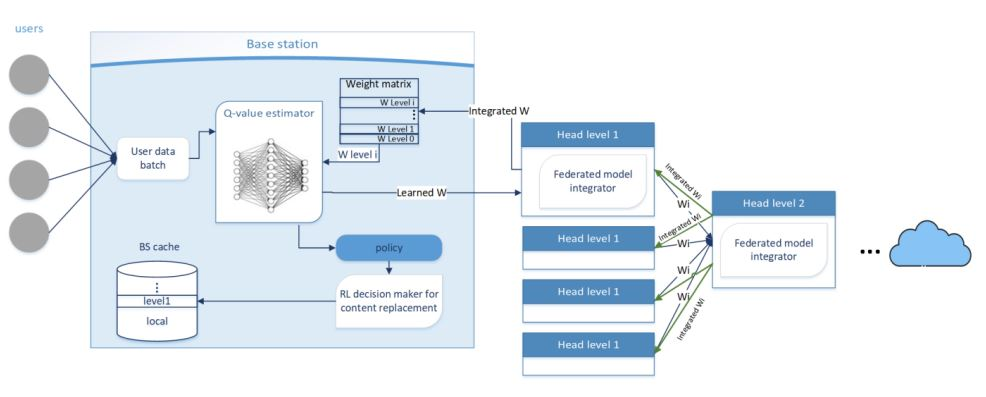
\includegraphics[width=15cm]{HFDRL}}
	\caption{مکانیزم تجمع مدل‌ها در معماری سلسله مراتبی فدراسیونی یادگیری تقویتی عمیق}
	\label{fig:hfdrl}
\end{figure}

 لازم به ذکر است که برای تعیین سرگروه، پارامترهایی چون زمان صرف شده برای دریافت محتوا با شناسه‌ی مشخص از دیتاسنتر تا گره مذکور، تعداد بارهایی که محتوا با شناسه‌ی مشخص از گره مذکور در خواست شده است و میزان حافظه‌ی لازم برای ذخیره‌ی محتوا، در نظر گرفته می‌شوند.
 
 پس از خوشه‌بندی گره‌ها در آغاز بازه‌ی زمانی،‌ هرگاه که ایستگاه پایه درخواستی را دریافت نماید، مراحل زیر را مطابق با شکل \ref{fig:fdrl} برای پاسخگویی دنبال می‌کند:
 \begin{enumerate}
 	\item 
 	در صورتیکه دیتا در حافظه‌ی محلی موجود باشد، به تعداد بارهای موفقیت آمیز در یافتن پاسخ از حافظه اضافه شده و در آخر نیز دیتا برای کاربر فراهم می‌گردد.
 	\item 
 	در صورتیکه محتوا در حافظه‌ی محلی موجود نباشد اما گره دیگری از خوشه آن را ذخیره کرده باشد، به تعداد بارهای موفقیت آمیز در یافتن پاسخ از حافظه اضافه شده و توسط ایستگاه پایه‌ی همگروه با آن دیتا برای کاربر ارسال می‌شود.
 	\item 
 	در صورتیکه محتوا در حافظه‌ی محلی و گره دیگری از خوشه موجود نباشد، درخواست به سطوح بالاتر رفته و در صورت موجود بودن به تعداد بارهای موفقیت آمیز در یافتن پاسخ از حافظه اضافه شده و توسط ایستگاه پایه‌ی مربوطه دیتا برای کاربر ارسال می‌شود.
 	\item 
 	در صورتیکه دیتا در حافظه‌ی محلی،‌ گره‌های خوشه و یا سطوح بالاتر وجود نداشته باشد، از دیتاسنتر مقدار مربوط به آن واکشی می‌شود. حال براساس میزان محاسبه شده برای محبوبیت محتوا دیتا در عمومی‌ترین لایه که حداقل میزان محبوبیت مربوط به آن را تأمین می‌نماید، ذخیره می‌گردد. 
 \end{enumerate}

\begin{figure}[ht]
	\centerline{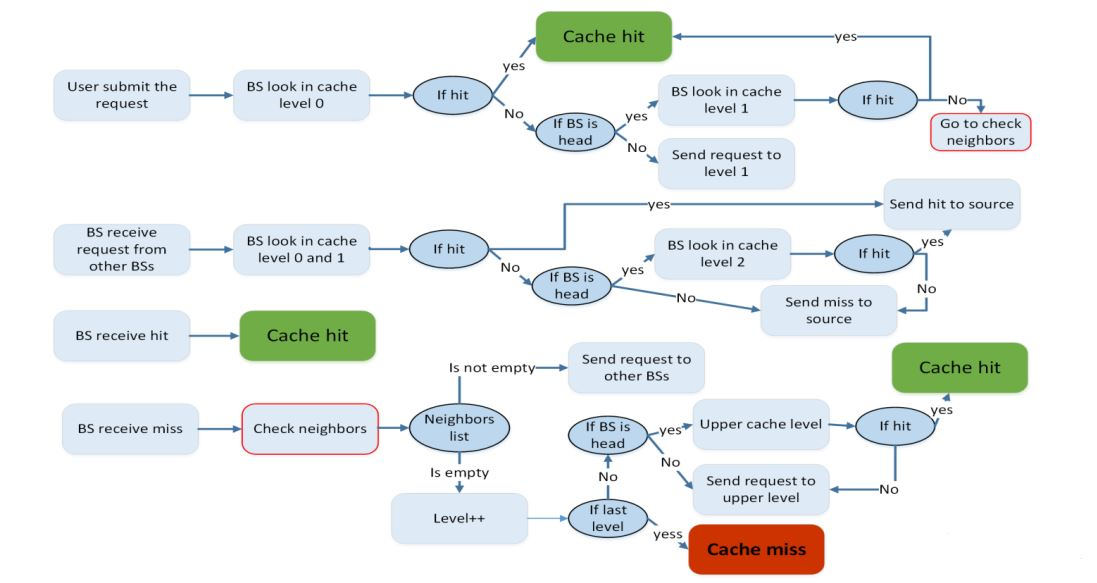
\includegraphics[width=15cm]{FDRL}}
	\caption{دیاگرام جریان داده برای پاسخ به درخواست‌های کاربران در مدل سلسله مراتبی و مشارکتی}
	\label{fig:fdrl}
\end{figure}

در آخر نیز دیده می شود که با خوشه‌بندی گره‌های لبه میزان موفقیت در ارسال پاسخ با ذخیره‌سازی افزایش می‌یابد. در این مقاله، لایه‌بندی‌ها نهایتاً تا سه لایه انجام می‌شود و کارآمدی استراتژی به کار رفته برای طبقه‌بندی سه لایه از طبقه‌بندی دولایه و برای طبقه‌بندی دو لایه نسبت به حالت تک لایه بیشتر می‌باشد.


		% فصول دوم: مروری بر مطالعات انجام شده
% !TeX root=../main.tex
\chapter{مشارکت در موضوع}

در ابتدا راهکارهای پیشنهادی در مقالات فصل 2 مورد بررسی قرار می‌گیرند، سپس با استفاده از آنها و در تکمیل راه‌حل‌های ارائه شده‌ی تا کنون، برای حل مسئله‌ی ذخیره‌سازی در شبکه‌ی اینترنت وسایل نقلیه استراتژی ذخیره‌سازی جدید و قابل قبولی ارائه می‌گردد. 
%\thispagestyle{empty} 

\section{نقدی بر مقالات فصل 2}
به طور کلی در هر دامنه‌ی تعریفی بزرگترین مشکلی که ‌یادگیری تقویتی عمیق با آن مواجه است، پایین بودن سرعت همگرایی به مقدار بهینه می‌باشد به علاوه‌ی اینکه تعامل با محیط برای تخمین میزان محبوبیت فایل‌ها هزینه دارد. جدای از این موارد، استفاده‌ی از شبکه‌ی عصبی باعث همگرایی به نقاط بهینه‌ی محلی می‌شود که با استفاده از تکنینک‌هایی می‌توان نقاط همگرایی را بهبود بخشید. به عنوان مثال در مقاله‌ی \cite{wu2021caching} با استفاده از الگوریتم \lr{Bootstrapped DQN} به جای \lr{Double DQN} یا \lr{DQN}، می توان متوسط پاداش‌های دریافتی را با واریانس کمتری تخمین زد. 

در واقع در الگوریتم \lr{Bootstrapped DQN} از چندین شبکه‌ی عصبی برای تخمین ارزش استیت-اکشن‌ها و یک بافر تجربیات استفاده می‌شود. برای تخمین ارزش استیت-اکشن‌ها، تجربیات تا این لحظه به عنوان ورودی بین شبکه‌های عصبی تقسیم می‌شود و خروجی‌های مربوط به آن از طریق یک شبکه‌ی مشترک بین شبکه‌های عصبی ارزیابی شده و به این ترتیب ارزش استیت-اکشن‌ها به مقادیر محلی بهینه‌تری همگرا می‌شود. در شکل \ref{fig:bootstrappeddqn} که برگرفته از مقاله‌ی \cite{osband2016deep} می‌باشد، دیاگرام مربوط به این الگوریتم را مشاهده می‌کنید.

\begin{figure}[ht]
	\centerline{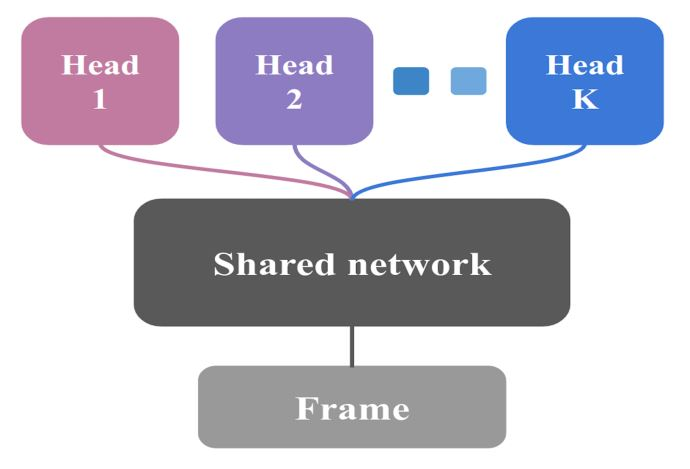
\includegraphics[width=6cm]{bootdqn}}
	\caption{دیاگرام الگوریتم \lr{Bootstrapped DQN}}
	\label{fig:bootstrappeddqn}
\end{figure}

\newpage
استفاده از خوشه‌بندی مطابق با آنچه که در مقاله‌ی \cite{majidi2021hfdrl} آورده شده است یا با استفاده از معماری ریشه-برگ در مقاله‌ی \cite{wu2022deep} با توجه به توپولوژی شبکه، می‌تواند تنوع محتویات کش شده در حافظه‌ی گره‌های لبه را در محیط‌های تعاملی چندعامله افزایش دهد و بنابراین میزان موفقیت حافظه‌ی کش در تأمین دیتای درخواستی نیز افزایش می‌یابد. البته در این مقالات درباره‌ی نحوه‌ی آپدیت خوشه‌بندی‌های موجود صحبتی به میان نیامده حال آنکه یکی از ویژگی‌هایی که در خوشه‌بندی لحاظ می‌شود الگوی درخواستی کاربران است و با توجه به غیرایستان بودن محیط، این الگو با زمان تغییر می‌یابد و لازم است تا خوشه‌بندی‌ها نیز آپدیت شوند که در بخش بعدی راه حلی برای رویارویی با این چالش ارائه می‌شود.

\section{بیان مشارکت}
طبیعت محیط در انتخاب الگوریتم یادگیری تقویتی مناسب برای تخمین میزان محبوبیت فایل‌ها تأثیر به سزایی دارد. به عنوان مثال در مقاله‌ی \cite{qiao2019deep} دیدیم که در نظر گرفتن حرکت گره‌های مصرف کننده در شبکه‌های اینترنت اشیا، بر تعریف مجموعه‌ی استیت‌ها و اکشن‌ها اثر ‌می‌گذارد و نیز دیدیم که مقاله  روشی را برای تخمین سیاست بهینه به طور مستقیم ارائه کرده بود. حال برای شبیه‌سازی شبکه‌های اینترنت وسایل نقلیه، استفاده از سیمولاتوری مانند \lr{OMNET++} برای شبیه‌سازی شبکه‌ی هدف و عامل‌های به کار رفته در محیط، می‌تواند راهگشا باشد.

علاوه بر این برای حل مشکل سرعت همگرایی استفاده از الگوریتم \lr{Penalized NFAC (PeNFAC)} که در مقاله‌ی  \cite{zimmer2019exploiting} معرفی شده است به جای  \lr{DDPG}، می‌تواند به ما در تخمین مستقیم سیاست بهینه کمک کند. در مقاله‌ی \cite{zimmer2019exploiting} کارکرد دو الگوریتم نامبرده با یکدیگر مقایسه شده است و دیده می‌شود که سرعت همگرایی \lr{PeNFAC} نسبت به \lr{DDPG} به سیاست بهینه بیشتر بوده و در ضمن مجموع پاداش‌های دریافتی در \lr{PeNFAC} نسبت به \lr{DDPG} به مقدار بیشتری همگرا می‌گردد و از الگوریتم \lr{PeNFAC} در حالت‌های کنترلی متمرکز و غیرمتمرکز می‌توان استفاده نمود.

در ادامه برای آپدیت خوشه بندی‌های مبتنی بر الگوریتم \lr{K-means} در استراتژی ذخیره سازی چندعامله در محیط شبکه‌های اینترنت وسایل نقلیه، از متدهای مربوط به \lr{Transfer Learning} می‌توان استفاده کرد. در واقع در این دسته از متدها از دانسته‌های قبلی برای آپدیت مدل برای تسک جدید (که در اینجا هایپر پارامتر \lr{K} با توجه به شرایط جدید محیطی آپدیت می‌شود.) استفاده می‌شود. 

در مسئله‌ی بهینه سازی مطرح شده، تابع هدف ما کاهش تابع هزینه‌ی وزندار حاصل از سه پارامتر مصرف انرژی در حسگرها، طول عمر دیتا (مدت زمانی که از اعتبار دیتا گذشته) و ترافیک لینک های پشتی می‌باشد.
		% فصل سوم: روش تحقیق
% !TeX root=../main.tex
\chapter{بحث و نتیجه‌گیری}
%\thispagestyle{empty} 
به طور کلی با توجه به ماهیت متمایز شبکه‌های اینترنت اشیا نسبت به سایر شبکه‌های مبتنی بر محتوا، استراتژی ذخیره‌سازی در این شبکه‌ها با چالش‌هایی روبه‌روست. از مهمترین چالش‌های پیش رو یکی مدت زمان محدود اعتبار داده و دیگری غیرایستان بودن توزیع محبوبیت فایل‌ها در محیط می‌باشد. علاوه بر این محیطی که استراتژی ذخیره‌سازی برای آن طراحی ‌می‌شود، در انتخاب الگوریتم و یا رویه‌ی ذخیره‌سازی اثر می‌گذارد. به عنوان مثال در صورتی‌که حرکت افزاره‌ها در شبکه‌های اینترنت اشیا قابل اغماض نباشد، فضای اکشن‌ها دیگر پیوسته نبوده و این مسئله تخمین ما از ارزش استیت‌ها و یا استیت-اکشن‌ها را دچار خطا می‌کند و بنابراین به طور مستقیم با استفاده از الگوریتم‌های متناظر به طور مستقیم سیاست بهینه را تخمین می‌زنیم. 

در محیط مسئله به تعداد گره‌های لبه در شبکه اینترنت اشیا، عامل تعریف می‌نماییم. هر چه میزان تنوع در محتویات ذخیره شده‌ی بین عامل‌ها تا حد معقولی بیشتر شود، عملاً استراتژی ذخیره‌سازی کارآمدتر خواهد بود. بدین منظور لازم است تا پردازنده‌ای داشته باشیم که به طور مشترک به گره‌های لبه برای ذخیره‌سازی یا جایگزینی محتوا در حافظه فرمان می‌دهد. حال هر چه این پردازنده به لایه‌ی کاربران نزدیکتر باشد یا حافظه‌ای برای ذخیره‌سازی محتوای مشترک داشته باشد،‌ عملاً استراتژی ذخیره‌سازی موفقیت‌آمیزتر خواهد بود که برای تحقق این امر می توان به روش‌های مختلف گره‌های در لایه‌ی لبه را خوشه‌بندی کرد.		% فصل چهارم: نتایج
%% !TeX root=../main.tex
\chapter{بحث و نتیجه‌گیری}
%\thispagestyle{empty} 
\section{مقدمه}
تاکنون شما در پایان‌نامه‌ای که مشغول نوشتن آن هستید، پاسخ چهار سؤال را داده‌اید:
\begin{itemize}
	\item
	چرا تحقیق را انجام دادید؟ (مقدمه)
	\item
	دیگران در این زمینه‌ چه کارهایی کرده‌اند و تمایز کار شما با آنها؟ (مرور ادبیات)
	\item
	چگونه تحقیق را انجام دادید؟ (روش‌ها)
	\item
	چه از تحقیق به دست آوردید؟ (یافته‌ها)
\end{itemize}
حال زمان آن فرا رسیده که با توجه به تمامی مطالب ذکر شده، در نهایت به سؤال آخر پاسخ دهید:
\begin{itemize}
	\item
	چه برداشتی از یافته‌های تحقیق کردید؟ (نتیجه‌گیری)
\end{itemize}
در واقع در این بخش، هدف، پاسخ به این سوال است که چه برداشتی از یافته‌ها کردید و این یافته‌ها چه فایده‌ای دارند؟

نتیجه‌گیری مختصری بنویسید. ارائهٔ داده‌ها، نتایج و یافته‌ها در فصل چهارم ارائه می‌شود. در این فصل تفاوت، تضاد یا تطابق بین نتایج تحقیق با نتایج دیگر محققان باید ذکر شود.
\emph{تفسیر و تحلیل نتایج نباید بر اساس حدس و گمان باشد}،
بلکه باید
\textbf{برمبنای نتایج عملی استخراج‌شده}
از تحقیق و یا
\textbf{استناد به تحقیقات دیگران}
باشد.
با توجه به حجم و ماهیت تحقیق و با صلاحدید استاد راهنما، این فصل می‌تواند تحت عنوانی دیگر بیاید یا به دو فصل جداگانه با عناوین مناسب، تفکیک شود. این فصل فقط باید به جمع‌بندی دست‌آوردهای فصل‌های سوم و چهارم محدود و از ذکر موارد جدید در آن خودداری شود. در عنوان این فصل، به جای کلمهٔ «تفسیر» می‌توان از واژگان «بحث» و «تحلیل» هم استفاده کرد. این فصل شاید مهم‌ترین فصل پایان‌نامه باشد.

در این فصل خلاصه‌ای از یافته‌های تحقیق جاری ارائه می‌شود. این فصل می‌تواند حاوی یک مقدمه، شامل مروری اجمالی بر مراحل انجام تحقیق باشد (حدود یک صفحه). مطالب پاراگراف‌بندی شود و هر پاراگراف به یک موضوع مستقل اختصاص یابد. فقط به ارائهٔ یافته‌ها و دست‌آوردها بسنده شود و
\emph{از تعمیم بی‌مورد نتایج خودداری شود.}
تا حد امکان از ارائهٔ 
\emph{جداول و نمودارها در این فصل اجتناب شود.}
از ارائهٔ 
\emph{عناوین کلی}
در حوزهٔ تحقیق و قسمت پیشنهاد تحقیقات آتی خودداری شود و کاملاً در چارچوب و زمینهٔ مربوط به تحقیق جاری باشد. این فصل حدود ۱۰-۱۵ صفحه است.

\section{محتوا}
به ترتیب شامل موارد زیر است:

\subsection{جمع‌بندی}
خلاصه‌ای از تمام یافته‌ها و دست‌آوردهای تحقیق جاری است.

\subsection{نوآوری}
این قسمت، نوآوری تحقیق را بر اساس یافته‌های آن تشریح می‌کند. که دارای دو بخش اصلی است:
\begin{enumerate}
	\item
	نوآوری تئوری، یعنی تمایز تئوریک کار با کارهای محققین قبلی.
	\item
	نوآوری عملی، یعنی توصیه‌های محقق به صنعت برای بهبود بخشیدن به کارها، بر اساس یافته‌های تحقیق.
\end{enumerate}

\subsection{پیشنهادها}
این بخش، عناوین و موضوعات پیشنهادی را برای تحقیقات آتی،
\emph{بیشتر در زمینهٔ مورد بحث در آینده}
ارائه می‌کند.

\subsection{محدودیت‌ها}
در اینجا انواع محدودیت‌های تحقیق تشریح می‌شوند؛ از جمله، محدودیت‌هایی که کنترل آن از عهده محقق خارج است، مانند انتخاب نوع یافته‌ها؛ و همچنین دیگر محدودیت‌هایی که کنترل آن در دست محقق است، مانند موضوع و محل تحقیق و ... . تأثیر این محدودیت‌ها بر یافته‌های تحقیق در این قسمت شرح داده می‌شوند.		% فصل پنجم: بحث و نتیجه‌گیری

% مراجع
% اگر از استیل‌های natbib استفاده می‌کنید باید دو خط را در فایل commands.tex تغییر دهید.
\pagestyle{empty}
{
\small
\onehalfspacing
\bibliographystyle{plain-fa} % or plainnat-fa for author-date
\bibliography{./tex/MyReferences}
}

\pagestyle{fancy}

%\appendix
% فصلهای پس از این قسمت به عنوان ضمیمه خواهند آمد.

% دستورات لازم برای تبدیل «فصل آ» به «پیوست آ» در فهرست مطالب
%\addtocontents{toc}{
    %\protect\renewcommand\protect\cftchappresnum{\appendixname~}%
    %\protect\setlength{\cftchapnumwidth}{\mylenapp}}
    
% دستورات لازم برای شماره‌گذاری صفحات پیوست‌ها بشکل آ-۱ (فعلا با glossaries سازگار نیست)
% \let\Chapter\chapter
%\pretocmd{\chapter}{
%  \clearpage
%  \pagenumbering{arabic}
%  \renewcommand*{\thepage}{\rl{\thechapter-\arabic{page}}}}{}{}
%%%%%%%%%%%%%%%%%%%%%%%%%%%%%%%%%%%%%
        

%% !TeX root=../main.tex

\chapter{آشنایی سریع با برخی دستورات لاتک}
\label{app:latexIntro}
%\thispagestyle{empty}
در این فصل ویژگی‌های مهم و پرکاربرد زی‌پرشین و لاتک معرفی می‌شود. برای راهنمایی بیشتر و به‌کاربردن ویژگی‌های پیشرفته‌تر به راهنمای زی‌پرشین و راهنمای لاتک مراجعه کنید. برای آگاهی از دستورات لاتک که این خروجی را تولید کرده‌اند فایل \lr{appendix1.tex} را ملاحظه فرمایید.
\footnote{بیشتر مطالب این بخش از مثال 
\lr{xepersian\_example.tex}
گرفته شده‌اند که توسط آقای امیرمسعود پورموسی آماده شده است.}

\section{بندها و زیرنویس‌ها}
هر جایی از نوشتهٔ خود، اگر می‌خواهید به سر سطر بروید و یک بند (پاراگراف) تازه را آغاز کنید، باید یک خط را خالی بگذارید%
\footnote{یعنی دوبار باید کلید \lr{Enter} را بزنید.}
 مانند این:

حالا که یک بند تازه آغاز شده است، یک زیرنویس انگلیسی%
\LTRfootnote{English Footnote!}
 هم می‌نویسیم!
\section{فرمول‌های ریاضی}
\label{formula}

اینجا هم یک فرمول می‌آوریم که شماره دارد:
\begin{equation}\label{eq:yek}
A=\frac{c}{d}+\frac{q^2}{\sin(\omega t)+\Omega_{12}}
\end{equation}
در لاتک می‌توان به کمک فرمان 
\lr{\textbackslash label\{\}}
به هر فرمول یک نام نسبت داد. در فرمول بالا نام \lr{eq:yek} را برایش گذاشته‌ایم (پروندهٔ \lr{tex} همراه با این مثال را ببینید). این نام ما را قادر می‌کند که بعداً بتوانیم با فرمان
\lr{\textbackslash ref\{eq:yek\}}
به آن فرمول با شماره ارجاع دهیم. یعنی بنویسیم فرمول \ref{eq:yek}. 
لاتک خودش شمارهٔ این فرمول‌ها را مدیریت می‌کند.\footnote{یعنی اگر بعداً فرمولی قبل از این فرمول بنویسیم، خودبه‌خود شمارهٔ این فرمول و شمارهٔ ارجاع‌ها به این فرمول یکی زیاد می‌شود. دیگر نگران شماره‌گذاری فرمول‌های خود نباشید!} این هم یک فرمول که شماره ندارد:
$$A=|\vec{a}\times \vec{b}| + \sum_{n=0}^\infty C_{ij}$$

این هم عبارتی ریاضی مانند 
$\sqrt{a^2+b^2}$
 که بین متن می‌آید.
\subsection{یک زیربخش}
\label{zirbakhsh}

این زیربخش \ref{zirbakhsh} است؛ یعنی یک بخش درون بخش \ref{formula} است.
\subsubsection{یک زیرزیربخش}
این هم یک زیرزیربخش است. در لاتک می‌توانید بخش‌های تودرتو در نوشته‌تان تعریف کنید تا ساختار منطقی نوشته را به خوبی نشان دهید. می‌توانید به این بخش‌ها هم با شماره ارجاع دهید، مثلاً بخش فرمول‌های ریاضی شماره‌اش \ref{formula} است.
\section{نوشته‌های فارسی و انگلیسی مخلوط}
نوشتن یک کلمهٔ انگلیسی بین متن فارسی بدیهی است، مانند Example در این جمله.\footnote{هرچند بهتر است باز هم آن کلمه را مانند \lr{Example} در این جمله بنویسید.}
نوشتن یک عبارت چندکلمه‌ای مانند
 \lr{More than one word} کمی پیچیده‌تر است.

اگر ناگهان تصمیم بگیرید که یک بند کاملاً انگلیسی را بنویسید، باید:
\begin{latin}
This is an English paragraph from left to right. You can write as much as you want in it.
\end{latin}
\section{افزودن تصویر به نوشته}
پروندهٔ تصویر دلخواه خود را در کنار پروندهٔ \lr{tex} قرار دهید. سپس به روش زیر تصویر را در نوشتهٔ خود بیاورید:
\begin{latin}
\begin{verbatim}
\includegraphics{YourImageFileName}
\end{verbatim}
\end{latin}
به تصویرها هم مانند فرمول‌ها و بخش‌ها می‌توان با شماره ارجاع داد. مثلاً تصویر \ref{fig:shir} یک شیر علاقه‌مند به لاتک را در حال دویدن نشان می‌دهد. برای جزئیات بیشتر دربارهٔ روش گذاشتن تصویرها در نوشته باید راهنماهای لاتک را بخوانید.
\begin{figure}[ht]
\centerline{
\includegraphics[width=5cm]{lion}}
\caption{در این تصویر یک شیر علاقه‌مند به لاتک را در حال دویدن می‌بینید.}
\label{fig:shir}
\end{figure}

به تصویرها هم مانند فرمول‌ها و بخش‌ها می‌توان با شماره ارجاع داد. مثلاً تصویر بالا شماره‌اش \ref{fig:shir} است. برای جزئیات بیشتر دربارهٔ روش گذاشتن تصویرها در نوشته باید راهنماهای لاتک را بخوانید.

\section{محیط‌های شمارش و نکات}
برای فهرست‌کردن چندمورد، اگر ترتیب برایمان مهم نباشد:
\begin{itemize}
\item مورد یکم
\item مورد دوم
\item مورد سوم
\end{itemize}
و اگر ترتیب برایمان مهم باشد:
\begin{enumerate}
\item مورد یکم
\item مورد دوم
\item مورد سوم
\end{enumerate}
می‌توان موردهای تودرتو داشت:
\begin{enumerate}
\item مورد ۱
\item مورد ۲
\begin{enumerate}
\item مورد ۱ از ۲
\item مورد ۲ از ۲
\item مورد ۳ از ۲
\end{enumerate}
\item مورد ۳
\end{enumerate}
شماره‌گذاری این موردها را هم لاتک انجام می‌دهد.

\section{تعریف و قضیه}
برای ذکر تعریف، قضیه و مثال مثالهای ذیل را ببینید.
\begin{definition}
مجموعه همه ارزیابی‌های  (پیوسته)  روی $(X,\tau)$، دامنه توانی احتمالی
\index{دامنه توانی احتمالی}
$ X $
نامیده می‌شود.
\end{definition}
\begin{theorem}[باناخ-آلااغلو]
\index{قضیه باناخ-آلااغلو}
اگر $ V $ یک همسایگی $ 0 $ در فضای برداری 
\index{فضای!برداری}
 توپولوژیکی $ X $ باشد و 
\begin{equation}\label{eq1}
K=\left\lbrace \Lambda \in X^{*}:|\Lambda x|\leqslant 1 ; \ \forall x\in V\right\rbrace,
\end{equation}
آنگاه $ K $،  ضعیف*-فشرده است که در آن، $ X^{*} $ دوگان
\index{فضای!دوگان}
 فضای برداری توپولوژیکی $ X $ است به ‌طوری که عناصر آن،  تابعی‌های 
خطی پیوسته
\index{تابعی خطی پیوسته}
 روی $X$ هستند.
\end{theorem}
تساوی \eqref{eq1} یکی از مهم‌ترین تساوی‌ها در آنالیز تابعی است که در ادامه، به وفور از آن استفاده می‌شود.
\begin{example}
برای هر فضای مرتب، گردایه 
$$U:=\left\lbrace U\in O: U=\uparrow U\right\rbrace $$
از مجموعه‌های بالایی باز، یک توپولوژی تعریف می‌کند که از توپولوژی اصلی، درشت‌تر  است.
\end{example}
حال تساوی 
\begin{equation}\label{eq2}
\sum_{n=1}^{+\infty} 3^{n}x+7x=\int_{1}^{n}8nx+\exp{(2nx)}
\end{equation}
را در نظر بگیرید. با مقایسه تساوی \eqref{eq2} با تساوی \eqref{eq1} می‌توان نتیجه گرفت که ...


\section{چگونگی نوشتن و ارجاع به مراجع}
\label{Sec:Ref}


در لاتک به راحتی می‌توان مراجع خود را نوشت و به آنها ارجاع داد. به عنوان مثال برای معرفی کتاب گنزالس \cite{Gonzalez02book} به عنوان یک مرجع می‌توان آنرا به صورت زیر معرفی نمود:

\singlespacing
\begin{LTR}
\begin{verbatim}
\bibitem{Gonzalez02book}
Gonzalez, R.C., and Woods, R.E. {\em Digital Image Processing}, 3rd ed..
Prentice-Hall, Inc., Upper Saddle River, NJ, USA, 2006.
\end{verbatim}
\end{LTR}
\doublespacing

در دستورات فوق \lr{Gonzalez02book}  برچسبی است که به این مرجع داده شده است و با استفاده از دستور 
\verb!\cite{Gonzalez02book}!
می‌توان به آن ارجاع داد؛ بدون این که شماره‌اش را در فهرست مراجع‌مان بدانیم.

اگر این اولین مرجع ما باشد در قسمت مراجع به صورت زیر خواهد آمد:\\
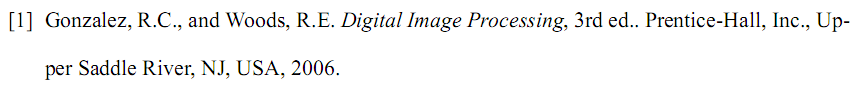
\includegraphics[width=\textwidth]{gonzalez.png}

این شیوهٔ تعریف مراجع بسیار ابتدایی است و اگر فرمت مراجع، ترتیب یا تعداد آنها را خواسته باشید تغییر دهید، به عنوان مثال ابتدا حرف اول نام نویسنده بیاید و سپس نام خانوادگی، باید همه کارها را به صورت دستی انجام دهید!
چون در یک \پ یا مقاله باید کنترل کاملی بر مراجع خود داشته باشید و به راحتی بتوانید قالب مراجع را عوض کنید، بنابراین می‌بایست از \lr{Bib\TeX} استفاده کنید که درپیوست  \ref{app:refMan} به  آن پرداخته خواهد شد.
		% پیوست اول: آشنایی مقدماتی با لاتک
%% !TeX root=../main.tex

\chapter{‌جدول، نمودار و الگوریتم در لاتک}
\label{app:latex:more}
%\thispagestyle{empty}

در این بخش نمونه مثالهایی از جدول، شکل، نمودار، الگوریتم و معادلات ریاضی را در لاتک خواهیم دید.
دقت کنید که در پایان‌نامه‌ها و مقالات، باید قاعدهٔ «ارجاع به جلو%
\LTRfootnote{Forward Referencing}»
رعایت شود؛ یعنی ابتدا در متن به شمارهٔ شکل، جدول یا معادله اشاره شود و بعد از آن (زیر آن) خود شکل، جدول یا معادله رسم شود. (توضیحات بیشتر در قسمت
\ref{sec:floatObjs}).

\section{جدول}
دستور اصلی برای رسم جدول در لاتک 
\verb|tabular|
می‌باشد که جدول
\eqref{tab:motionModels}
با استفاده از آن کشیده شده است؛ در
\verb|tabular|
عرض جدول برابر با مجموع عرض ستون‌ها و حداکثر مساوی عرض متن است.
\begin{table}[ht]
\caption{مدلهای تبدیل.}
\label{tab:motionModels}
\centering
\onehalfspacing
\begin{tabular}{|r|c|l|r|}
	\hline نام مدل & درجه آزادی & تبدیل مختصات & توضیح \\ 
	\hline انتقالی & ۲ & $\begin{aligned} x'=x+t_x \\ y'=y+t_y \end{aligned}$  &  انتقال دوبعدی\\ 
	\hline اقلیدسی & ۳ & $\begin{aligned} x'=x\cos\theta - y\sin\theta+t_x \\ y'=x\sin\theta+y\cos\theta+t_y \end{aligned}$  &  انتقالی+دوران \\ 
	\hline 
\end{tabular} 
\end{table}

برای اینکه عرض جدول قابل کنترل باشد، باید از دستورات
\verb|tabularx|،
\verb|tabulary| یا
\verb|tabu|
استفاده کرد که راهنمای آنها در اینترنت وجود دارد.
مثلاً جدول
\ref{tab:motionModelsCont}
با
\verb|tabularx|
رسم شده که عرض جدول در آن ثابت بوده و ستون‌های از نوع
\verb|X|
عرض خالی جدول را پر می‌کنند.
\begin{table}[ht]
	\caption{مدلهای تبدیل دیگر.}
	\label{tab:motionModelsCont}
	\centering
	\onehalfspacing
	\begin{tabularx}{\textwidth}{|r|c|l|X|}
		\hline نام مدل & درجه آزادی & تبدیل مختصات & توضیح \\ 
		\hline مشابهت & ۴ & $\begin{aligned} x'=sx\cos\theta - sy\sin\theta+t_x \\ y'=sx\sin\theta+sy\cos\theta+t_y  \end{aligned}$  & اقلیدسی+تغییرمقیاس \\ 		
		\hline آفین & ۶ & $\begin{aligned} x'=a_{11}x+a_{12}y+t_x \\ y'=a_{21}x+a_{22}y+t_y \end{aligned}$  & مشابهت+اریب‌شدگی \\
		\hline
	\end{tabularx}
\end{table}

\section{معادلات ریاضی و ماتریس‌ها}
تقریباً هر آنچه دانشجویان برای نوشتن فرمول‌های ریاضی لازم دارند، در کتاب 
\lr{mathmode}
آمده است. کافیست در خط فرمان، دستور زیر را وارد کنید:
\begin{latin}
	\texttt{texdoc mathmode}
\end{latin}
متن زیر شامل انواعی از اشیاء ریاضی است که با ملاحظه کدش می‌توانید با دستورات آن آشنا شوید.\\
شناخته‌شده‌ترین روش تخمین ماتریس هوموگرافی الگوریتم تبدیل خطی مستقیم (\lr{DLT\LTRfootnote{Direct Linear Transform}}) است.  فرض کنید چهار زوج نقطهٔ متناظر در دو تصویر در دست هستند،  $\mathbf{x}_i\leftrightarrow\mathbf{x}'_i$   و تبدیل با رابطهٔ
  $\mathbf{x}'_i = H\mathbf{x}_i$
  نشان داده می‌شود که در آن:
\[\mathbf{x}'_i=(x'_i,y'_i,w'_i)^\top  \]
و
\[ H=\left[
\begin{array}{ccc}
h_1 & h_2 & h_3 \\ 
h_4 & h_5 & h_6 \\ 
h_7 & h_8 & h_9
\end{array} 
\right]\]
رابطه زیر را برای الگوریتم  \eqref{alg:DLT} لازم داریم.
\begin{equation}
\label{eq:DLT_Ah}
\left[
\begin{array}{ccc}
	0^\top & -w'_i\mathbf{x}_i^\top & y'_i\mathbf{x}_i^\top \\ 
	w'_i\mathbf{x}_i & 0^\top & -x'_i\mathbf{x}_i^\top \\ 
	- y'_i\mathbf{x}_i^\top & x'_i\mathbf{x}_i^\top & 0^\top
\end{array} 
\right]
\left(
\begin{array}{c}
	\mathbf{h}^1 \\ 
	\mathbf{h}^2 \\ 
	\mathbf{h}^3
\end{array} 
\right)=0
\end{equation}

\section{الگوریتم}

\subsection{الگوریتم ساده با دستورهای فارسی}
با مفروضات فوق، الگوریتم \lr{DLT} به صورت نشان داده شده در الگوریتم \eqref{alg:DLT}  خواهد بود.
\begin{algorithm}[ht]
\onehalfspacing
\caption{الگوریتم \lr{DLT} برای تخمین ماتریس هوموگرافی.} \label{alg:DLT}
\begin{algorithmic}[1]
\REQUIRE $n\geq4$ زوج نقطهٔ متناظر در دو تصویر 
${\mathbf{x}_i\leftrightarrow\mathbf{x}'_i}$،\\
\ENSURE ماتریس هوموگرافی $H$ به نحوی‌که: 
$\mathbf{x}'_i = H \mathbf{x}_i$.
  \STATE برای هر زوج نقطهٔ متناظر
$\mathbf{x}_i\leftrightarrow\mathbf{x}'_i$ 
ماتریس $\mathbf{A}_i$ را با استفاده از رابطهٔ \ref{eq:DLT_Ah} محاسبه کنید.
  \STATE ماتریس‌های ۹ ستونی  $\mathbf{A}_i$ را در قالب یک ماتریس $\mathbf{A}$ ۹ ستونی ترکیب کنید. 
  \STATE تجزیهٔ مقادیر منفرد \lr{(SVD)}  ماتریس $\mathbf{A}$ را بدست آورید. بردار واحد متناظر با کمترین مقدار منفرد جواب $\mathbf{h}$ خواهد بود.
  \STATE  ماتریس هوموگرافی $H$ با تغییر شکل $\mathbf{h}$ حاصل خواهد شد.
\end{algorithmic}
\end{algorithm}

\subsection{الگوریتم پیچیده و تودرتو با دستورهای فارسی}
الگوریتم \ref{alg:simulation-random}، یک الگوریتم ترکیبی و تودرتو است که با کمک دستورهای بستهٔ \lr{algorithmic} نوشته شده است.

\begin{algorithm}[p]
    \onehalfspacing
    \caption{الگوریتم اجرای برنامهٔ شبیه‌سازی}
    \label{alg:simulation-random}
    \begin{algorithmic}[1]
        \REQUIRE زمان $t_{max}$ به عنوان زمان لازم برای انجام شبیه سازی،\\
        \REQUIRE  گراف شبکه برای شبیه سازی،
        \ENSURE جدول تغییرات گراف از لحظهٔ ۰ تا t.
        \FOR {تمام لحظات در بازهٔ ۰ تا $t_{max}$}
            \FOR {تمام پیوند‌ها}
                \STATE محاسبهٔ ضریب و نرخ انتقال پیوند
                \STATE محاسبهٔ کیفیت و نرخ یادگیری
            \ENDFOR
            \FOR {تمام گره‌ها}
                \STATE محاسبهٔ نرخ انتقال گره
                \STATE محاسبهٔ وضعیت جدید
            \ENDFOR
            \IF {تغییرات از مقدار $\delta$ کمتر است}
                \STATE شکستن حلقه
                \COMMENT{این شرط برای پایان قبل از رسیدن به محدودیت زمانی است، اگر تغییرات کمتر از $\delta$ باشد}
            \ELSIF {زمان اجرای برنامه بیش از حد طول کشیده \AND $t>100$}
                \STATE شکستن حلقه
            \ENDIF
        \ENDFOR
        \PRINT {زمان اجرای برنامه}
        \RETURN {ماتریس تغییرات زمانی}
    \end{algorithmic}
\end{algorithm}

\subsection{الگوریتم با دستورهای لاتین}
الگوریتم \ref{alg:RANSAC} یک الگوریتم با دستورهای لاتین است.

\begin{algorithm}[ht]
\onehalfspacing
\caption{الگوریتم \lr{RANSAC} برای تخمین ماتریس هوموگرافی.} \label{alg:RANSAC}
\begin{latin}
\begin{algorithmic}[1]
\REQUIRE $n\geq4$ putative correspondences, number of estimations, $N$, distance threshold $T_{dist}$.\\
\ENSURE Set of inliers and Homography matrix $H$.
\FOR{$k = 1$ to $N$}
  \STATE Randomly choose 4 correspondence,
  \STATE Check whether these points are colinear, if so, redo the above step
  \STATE Compute the homography $H_{curr}$ by DLT algorithm from the 4 points pairs,
  \STATE $\ldots$ % الگوریتم کامل نیست
  \ENDFOR
  \STATE Refinement: re-estimate H from all the inliers using the DLT algorithm.
\end{algorithmic}
\end{latin}
\end{algorithm}

\section{کد}
درج کد به زبان‌های مختلف به سادگی امکان‌پذیر است. برنامه
\ref{code:matlabEx}
یک قطعه کد
\lr{MATLAB}
را نشان می‌دهد.
\begin{figure}[ht]
	\begin{LTR}
        \singlespacing
		\lstinputlisting[language=MATLAB, caption={نمونه کد \lr{MATLAB}}, label={code:matlabEx}]{MatlabExample.m}
        % \doublespacing
	\end{LTR}
\end{figure}

\section{تصویر}
نمونهٔ یک تصویر را در فصل قبل دیدیم. دو تصویر شیر کنار هم را نیز در شکل
\ref{fig:twoLion}
مشاهده می‌کنید.
\begin{figure}[ht]
\centering 
\subfloat[شیر ۱]{ \label{fig:twolion:one}

\includegraphics[width=0.3\textwidth]{lion}}
%\hspace{2mm}
\subfloat[شیر ۲]{ \label{fig:twolion:two}

\includegraphics[width=0.3\textwidth]{lion}}%
\caption{دو شیر}
\label{fig:twoLion} %% label for entire figure
\end{figure}

\section{نمودار}
لاتک بسته‌هایی با قابلیت‌های زیاد برای رسم انواع مختلف نمودارها دارد. مانند بسته‌های \lr{Tikz} و  \lr{PSTricks}. توضیح اینها فراتر از این پیوست کوچک است.%
\footnote{
مثال‌هایی از بکارگیری بسته
\lr{Tikz}
را می‌توانید در
\url{http://www.texample.net/tikz/examples/}
ببینید. توصیه می‌شود دانشجویانی که قصد درج اشکالی مانند گراف را در سند خود دارند، مثالهایی از سایت مذکور را ملاحظه فرمایند.
}
یک نمودار رسم شده با بستهٔ 
\lr{TikZ}
 در شکل 
\ref{fig:parabola}
نشان داده شده است.
\begin{figure}[t]
\centering
\begin{tikzpicture}[scale=2.5]
  \shade[top color=blue,bottom color=gray!50] 
      (0,0) parabola (1.5,2.25) |- (0,0);
  \draw (1.05cm,2pt) node[above] 
      {$\displaystyle\int_0^{3/2} \!\!x^2\mathrm{d}x$};

  \draw[style=help lines] (0,0) grid (3.9,3.9)
       [step=0.25cm]      (1,2) grid +(1,1);

  \draw[->] (-0.2,0) -- (4,0) node[right] {$x$};
  \draw[->] (0,-0.2) -- (0,4) node[above] {$f(x)$};

  \foreach \x/\xtext in {1/1, 1.5/1\frac{1}{2}, 2/2, 3/3}
    \draw[shift={(\x,0)}] (0pt,2pt) -- (0pt,-2pt) node[below] {$\xtext$};

  \foreach \y/\ytext in {1/1, 2/2, 2.25/2\frac{1}{4}, 3/3}
    \draw[shift={(0,\y)}] (2pt,0pt) -- (-2pt,0pt) node[left] {$\ytext$};

  \draw (-.5,.25) parabola bend (0,0) (2,4) node[below right] {$x^2$};
\end{tikzpicture}
\caption{یک نمودار زیبا با ارقام فارسی و قابلیت بزرگ‌نمایی بسیار، بدون از دست دادن کیفیت.}
\label{fig:parabola}
\end{figure}

\section{نحوه قرارگیری اشیای شناور}
\label{sec:floatObjs}
شکل‌ها، جداول و الگوریتم‌ها در لاتک اشیای شناور محسوب می‌شوند؛ یعنی خود لاتک تصمیم می‌گیرد آنها را در کجای صفحه ترسیم کند تا زیباتر باشد. اما می‌توان به لاتک توصیه کرد که آن را در قسمت خاصی از صفحه رسم کند. برای اینکه قاعدهٔ «ارجاع به جلو» رعایت شود باید فقط از پرچم
\verb|[ht]|
استفاده کرد، که می‌گوید اگر جا شد شکل را دقیقاً در همین مکان و در غیراینصورت در بالای صفحه بعد رسم کن.
بنابراین دستورات درج تصویر، جدول و الگوریتم به صورت زیر باید باشند:

\begin{latin}
\begin{verbatim}
	\begin{figure/table/algorithm}[ht]
		...
	\end{figure/table/algorithm}
\end{verbatim}
\end{latin}
		% پیوست دوم: جدول، نمودار و الگوریتم در لاتک
%% !TeX root=../main.tex
\chapter{مراجع، واژه‌نامه و حاشیه‌نویسی}
\label{app:refMan}
%\thispagestyle{empty}

\section{مراجع و نقل‌قول‌ها}
\label{sec:refUsage}
منابعِ پایان‌نامه، پایه و اساس تحقیق شما به حساب می‌آیند و ضرورت انجام مطالعه و روش‌های به کار رفته در بسیاری از قسمت‌های آن، به کمک منابع صورت می‌گیرد. در استفاده از مراجع علمی در پایان‌نامه، باید سعی کنید بیشتر از
\textbf{منابع چاپ‌شده و مهم}
استفاده کنید و
\emph{ارجاع به داده‌های چاپ نشده، خلاصه‌ها و پایان‌نامه‌ها، سبب به‌هم‌خوردگی و کاهش اعتبار قسمت ارجاع منابع می‌شود.}
استفاده از منابع و نقل قول‌هایی به تحقیق شما ارزش می‌دهند که
\textbf{در راستای هدف تحقیق بوده و به آن اعتبار ببخشند.}
برخی از دانش‌جویان تصوّر می‌کنند که کثرت نقل‌قول‌ها و ارجاعات زیاد، مهم‌ترین معیار علمی شدن پایان‌نامه است؛ حال آنکه استناد به تعداد کثیری از منابع بدون مطالعه دقیق آنها و استفادهٔ مستقیم در پایان‌نامه، می‌تواند نشان‌دهندهٔ عدم احساس امنیت نویسنده باشد!

دو روش برای استفاده از نتایج، جملات، داده‌ها و روش‌های دیگران وجود دارد. یکی نقل‌قول مستقیم و دقیق است و دیگری استفاده غیرمستقیم در متن مقاله، که در ادامه به قواعد این دو نوع نقل‌قول و ارجاع‌دهی اشاره می‌کنیم:
\begin{description}
	\item[نقل‌قول مستقیم:]
	نقل‌قول مستقیم باید دقیق و بدون هیچ تغییری در جملات باشد. بهتر است این‌گونه نقل‌قول‌ها تا حد امکان کوتاه باشد. جملات کوتاه داخل گیومه قرار می‌گیرند و باید به منبع دقیق آن، طبق روش ارجاع‌دهی به منابع، اشاره شود. به عنوان مثال در
	\cite{persianbib87userguide}
	آمده است که:
	\begin{quote}
		«با استفاده از فیلد
		\lr{AUTHORFA}
		می‌توان معادل فارسی نام نویسندگان مقالات لاتین را در متن داشت. معمولاً در اسناد فارسی خواسته می‌شود که پس از ذکر معادل فارسی نام نویسنده، نام لاتین نویسنده(ها) به عنوان پاورقی درج شود
		\citep{persianbib87userguide}.»
	\end{quote}
	\item[نقل‌قول غیرمستقیم:]
	نقل‌قول غیرمستقیم به معنی استفاده از ایده‌ها، نتایج، روش‌ها و داده‌های دیگران در درون متنِ پایان‌نامه، ولی به سبک خودتان و متناسب و هماهنگ با روند پایان‌نامهٔ شماست. در این حالت نیز باید متناسب با شیوهٔ ارجاع‌دهی به آن استناد شود.
\end{description}

با توجه به وجود سبک‌های مختلف ارجاع‌دهی، باید
\textbf{روش قابل قبول و یکسانی}
در طول پایان‌نامه برای اشاره به مراجع در متن و همچنین تهیه فهرست مراجع در انتهای پایان‌نامه بکار رود. مثلاً برای پایان‌نامه‌های مهندسی می‌توان از سبک ارجاع‌دهی
\lr{IEEE}%
\LTRfootnote{\url{http://www.ieee.org/documents/ieeecitationref.pdf}}
یا
\lr{acm}
استفاده کرد. طبیعتاً باید تناظر یک‌به‌یک بین فهرست مراجع در انتهای گزارش و مراجع مورد استفاده در متن باشد%
\footnote{البته گاهی ممکن است محقق مرجعی را مورد مطالعه قرار داده لیکن در متن به آن اشاره نکرده باشد؛ برخی معتقدند در این موارد نیز آوردن آن در فهرست مراجع، اشکالی ندارد، به این شرط که از عنوان «فهرست منابع» به جای «فهرست مراجع» استفاده شود.}.

برای سهولت مدیریت مراجعِ \پ%
، اکیداً توصیه می‌شود از یک ابزار «مدیریت منابع» (با خروجی
\texorpdfstring{\lr{Bib\TeX}}{Bib\TeX}%
) همچون
\lr{Mendeley}،
\lr{Zotero},
\lr{EndNote}
یا
\lr{Citavi}
استفاده کنید.

\subsection{ مدیریت مراجع با  \texorpdfstring{\lr{Bib\TeX}}{Bib\TeX}}
در بخش \ref{Sec:Ref} اشاره شد که با دستور 
 \lr{\textbackslash bibitem}
  می‌توان یک مرجع را تعریف نمود و با فرمان
 \lr{\textbackslash cite}
  به آن ارجاع داد. این روش برای تعداد مراجع زیاد و تغییرات آنها مناسب نیست. برای مدیریت منابع زیاد، سه بستهٔ
\lr{BibTeX} (پیش‌فرض),
\lr{natbib}
(ارجاع‌دهی در متن به صورت نویسنده-سال)
و \lr{BibLaTeX} (جدید و منعطف‌پذیر)
وجود دارند. در ادامه توضیحاتی در مورد مدیریت منابع با \lr{BibTeX} و \lr{natbib} در زی‌پرشین خواهیم آورد که همراه با توزیع‌های معروف تِک عرضه می‌شوند
\footnote{روش \lr{BibLaTeX} هنوز برای متون فارسی به درستی ترجمه نشده است.}.

یکی از روش‌های قدرتمند و انعطاف‌پذیر برای نوشتن مراجعِ مقالات و مدیریت مراجع در لاتک، استفاده از  \lr{BibTeX} است.
 روش کار با بیب‌تک به این صورت است که مجموعهٔ همهٔ مراجعی را که در \پ استفاده کرده یا خواهیم کرد، 
در پروندهٔ جداگانه‌ای با پسوند
\lr{bib}
نوشته و به آن فایل در سند خودمان به صورت مناسب لینک می‌دهیم.
 کنفرانس‌ها یا مجله‌های گوناگون برای نوشتن مراجع، قالب‌ها یا قراردادهای متفاوتی دارند که به آنها استیل‌های مراجع گفته می‌شود.
 در این حالت به کمک ‌استیل‌های بیب‌تک خواهید توانست تنها با تغییر یک پارامتر در پروندهٔ ورودی خود، مراجع را مطابق قالب موردنظر تنظیم کنید. 
 بیشتر مجلات و کنفرانس‌های معتبر یک فایل سبک
 (\lr{BibTeX Style})
با پسوند \lr{bst} در وب‌گاه خود می‌گذارند که برای همین منظور طراحی شده است.

به جز نوشتن مقالات، این سبک‌ها کمک بسیار خوبی برای تهیهٔ مستندات علمی همچون پایان‌نامه‌هاست که فرد می‌تواند هر قسمت از کارش را که نوشت مراجع مربوطه را به بانک مراجع خود اضافه نماید. با داشتن چنین بانکی از مراجع، وی خواهد توانست به راحتی یک یا چند ارجاع به مراجع و یا یک یا چند بخش را حذف یا اضافه ‌نماید؛ 
مراجع به صورت خودکار مرتب شده و
\textbf{فقط مراجع ارجاع داده شده در قسمت کتاب‌نامه خواهندآمد.}
قالب مراجع به صورت یکدست مطابق سبک داده شده بوده و نیازی نیست که کاربر درگیر قالب‌دهی به مراجع باشد. 

\subsection{سبک‌های مورد تأیید دانشگاه تهران}
طبق «دستورالعمل نگارش و تدوین پایان‌نامه» دانشگاه تهران در
\cite{UTThesisGuide}،
ارجاع در متن می‌تواند مطابق با هر یک از دو الگوی هاروارد یا ونکوور باشد:
\singlespacing
\begin{description}
	\item[سیستم نویسنده-سال (هاروارد):]
	ذکر نام نویسنده و سال نشر در متن. در این الگو مراجع بر اساس حروف الفبا تنظیم می‌گردند.
	\item[سیستم شماره‌دار (ونکوور):]
	ارجاع به مراجع به کمک شماره در متن. در این الگو شماره هر مرجع به ترتیب ظاهر شدن آن در متن در داخل کروشه قرار می‌گیرد. فهرست مراجع نیز بر اساس شماره مرجع (نه حروف الفبا) تنظیم می‌گردد.
\end{description}
\doublespacing

در مدیریت منابع با
\lr{\textbf{BibTeX}}،
ارجاع‌ها در متن تنها به شکل
\textbf{شماره‌دار (ونکوور)}
امکان‌پذیر است، گرچه فهرست مراجع می‌تواند با روش‌های مختلف مرتب شود. اگر بخواهیم ارجاع‌ها در متن به صورت
\textbf{نویسنده-سال (هاروارد)}
باشد باید از بستهٔ
\lr{\textbf{natbib}}\LTRfootnote{Natural Sciences Citations \& References}
و استیل‌های مختلف آن استفاده کنیم.

هنگام استفاده از روش نویسنده-سال نوع پرانتزگذاری‌ها در وسط و انتهای جمله با هم فرق خواهد داشت. به مثال زیر مطابق با دستورالعمل
\cite{UTThesisGuide}
توجه کنید:

\textit{
ابتدا
\cite{Khalighi87xepersian}
بستهٔ زی‌پرشین را برای حروف‌چینی فارسی اختراع کرد. بعدها سبک‌های ارجاع‌دهی فارسی و قالب‌های پایان‌نامه نیز مبتنی بر آن ساخته شد
\citep{persianbib87userguide}.
ارجاع‌دهی به مراجع لاتین نیز در زی‌پرشین امکان‌پذیر است. مثلاً
\citelatin{Gonzalez02book}
یک کتاب انگلیسی است و به راحتی به مقالات انگلیسی نیز می‌توان ارجاع داد
\citeplatin{kim2016integrated}.}

در این مثال، ۴ ارجاع در وسط و انتهای جمله به مراجع فارسی و انگلیسی آمده است. وقتی از سیستم نویسنده-سال استفاده می‌کنید، بهتر است ارجاع‌های آخر جمله کلاً داخل پرانتر بیاید؛ بدین منظور باید به جای
\verb|\cite|
از
\verb|\citep|
استفاده کنید. اما در سیستم شماره‌دار چون تمام ارجاع‌ها داخل کروشه می‌آیند این امر اهمیت ندارد.\\
نمی‌توانید در متن فارسی، اسم لاتین محقق خارجی را بیاورید و برای جلوگیری از ایجاد ابهام، صرف‌نظر از نام لاتین هم مجاز نیست! توصیه می‌شود که نام محقق خارجی در متن با حروف فارسی و در پاورقی اسم تمام نویسندگان به صورت انگلیسی آورده شود. نحوهٔ رعایت این نکته را می‌توانید در کد مثال بالا ببینید.

گرچه در تمپلت ورد
\cite{UTThesisGuide}،
به صراحت ذکر شده که بهتر است برای پایان‌نامه‌های مهندسی از سبک 
\lr{IEEE}
استفاده شود (که از سیستم ونکوور تبعیت می‌کند)، اما ترتیب فهرست مراجع در
\lr{IEEE}
بر اساس ترتیب ارجاع در متن بوده و
\emph{مراجع انگلیسی و فارسی از هم تفکیک نمی‌شوند}
که متضاد با دستورالعمل
\cite{UTThesisGuide}
و نیز متضاد عرف اکثر پایان‌نامه‌های فارسی است.
بنابراین دقیقاً نمی‌توان سبک خاصی را برای مراجع پایان‌نامه‌های دانشگاه تهران اجبار کرد. مهم این است که
\textbf{سبک ارجاع‌دهی در تمام طول یک کتابچه}
(مثلاً پایان‌نامه، مقالات یک مجله یا کل یک کتاب) یکسان باشد. بهتر است
\textbf{بسته به حوزه پایان‌نامه}،
در این مورد با استاد راهنمای خود مشورت کنید.

\subsection{سبک‌های فارسی قابل استفاده در زی‌پرشین}
تعدادی از سبک‌های فارسی بسته
\lr{Persian-bib}%
\footnote{ برای اطلاع بیشتر به راهنمای بستهٔ
\lr{Persian-bib}
مراجعه فرمایید.}
که برای  زی‌پرشین آماده شده‌اند، عبارتند از:

\singlespacing
\begin{itemize}
\item \emph{سبک‌های شماره‌دار}:
	\begin{description}
	\item [unsrt-fa.bst] این سبک متناظر با \lr{unsrt.bst} می‌باشد. مراجع به ترتیب ارجاع در متن ظاهر می‌شوند.
	\item [plain-fa.bst] این سبک متناظر با \lr{plain.bst} می‌باشد. مراجع بر اساس نام‌خانوادگی نویسندگان، به ترتیب صعودی مرتب می‌شوند.
	 همچنین ابتدا مراجع فارسی و سپس مراجع انگلیسی خواهند آمد.
	\item [acm-fa.bst] این سبک متناظر با \lr{acm.bst} می‌باشد. شبیه \lr{plain-fa.bst} است.  قالب مراجع کمی متفاوت است. اسامی نویسندگان انگلیسی با حروف بزرگ انگلیسی نمایش داده می‌شوند. (مراجع مرتب می‌شوند)
	\item [ieeetr-fa.bst] این سبک متناظر با \lr{ieeetr.bst} می‌باشد. (مراجع مرتب نمی‌شوند)
	\end{description}
	
\item \emph{سبک‌های نویسنده-سال}:
	\begin{description}
	\item [plainnat-fa.bst] این سبک متناظر با \lr{plainnat.bst} می‌باشد. نیاز به بستهٔ \lr{natbib} دارد. (مراجع مرتب می‌شوند)
	\item [chicago-fa.bst] این سبک متناظر با \lr{chicago.bst} می‌باشد. نیاز به بستهٔ \lr{natbib} دارد. (مراجع مرتب می‌شوند)
	\item [asa-fa.bst] این سبک متناظر با \lr{asa.bst} می‌باشد. نیاز به بستهٔ \lr{natbib} دارد. (مراجع مرتب می‌شوند)
	\end{description}
\end{itemize}
\doublespacing

با استفاده از استیل‌های فوق می‌توانید به انواع مختلفی از مراجع فارسی و لاتین ارجاع دهید.
به عنوان مثال‌هایی از
\textbf{مراجع انگلیسی}،
مرجع
\cite{Baker02limits}\footnote{چون فیلد \lr{authorfa} برای این مرجع تعریف نشده در سبک نویسنده-سال با حروف لاتین به آن در متن ارجاع می‌شود که غلط است.}
مقالهٔ یک ژورنال، مرجع
\cite{Amintoosi09video}
مقالهٔ یک کنفرانس، مرجع
\citelatin{Gonzalez02book}
یک کتاب، مرجع
\cite{Khalighi07MscThesis}
پایان‌نامهٔ کارشناسی ارشد و مرجع
\citelatin{Borman04thesis}
یک رسالهٔ دکتری می‌باشد.\\
همچنین در میان
\textbf{مراجع فارسی},
مرجع
\cite{Vahedi87}
مقالهٔ یک مجله، مرجع
\cite{Amintoosi87afzayesh}
مقالهٔ یک کنفرانس، مرجع
\cite{Pedram80osool}
یک کتاب ترجمه‌شده با ذکر مترجمان و ویراستاران، مرجع
\cite{Pourmousa88mscThesis}
پایان‌نامهٔ کارشناسی ارشد%
\footnote{همان‌طور که در بخش
\ref{sec:refUsage}
اشاره شد، بهتر است زیاد از پایان‌نامه‌ها در مراجع استفاده نکنید.}،
مرجع
\cite{Omidali82phdThesis}
یک رسالهٔ دکتری و مراجع
\cite{persianbib87userguide, Khalighi87xepersian}
نمونه‌های متفرقه هستند.

\subsection{ساختار فایل مراجع}
برای استفاده از بیب‌تک باید مراجع خود را در یک فایل با پسوند \lr{bib} ذخیره نمایید. یک فایل \lr{bib} در واقع یک پایگاه داده از مراجع%
\LTRfootnote{Bibliography Database}
شماست که هر مرجع در آن به عنوان یک رکورد از این پایگاه داده
با قالبی خاص ذخیره می‌شود. به هر رکورد یک مدخل%
\LTRfootnote{Entry}
گفته می‌شود. یک نمونه مدخل برای معرفی کتاب \lr{Digital Image Processing} در ادامه آمده است:

\singlespacing
\begin{LTR}
\begin{verbatim}
@BOOK{Gonzalez02image,
  AUTHOR     = {Gonzalez,, Rafael C. and Woods,, Richard E.},
  TITLE      = {Digital Image Processing},
  PUBLISHER  = {Prentice-Hall, Inc.},
  YEAR       = {2006},
  ISBN       = {013168728X},
  EDITION    = {3rd},
  ADDRESS    = {Upper Saddle River, NJ, USA}
}
\end{verbatim}
\end{LTR}
\doublespacing

در مثال فوق، \lr{@BOOK} مشخصهٔ شروع یک مدخل مربوط به یک کتاب و \lr{Gonzalez02book} برچسبی است که به این مرجع منتسب شده است.
 این برچسب بایستی یکتا باشد. برای آنکه بتوان
\textbf{برچسب مراجع}
 را به راحتی به خاطر سپرد و حتی‌الامکان برچسب‌ها متفاوت با هم باشند، معمولاً از قوانین خاصی به این منظور استفاده می‌شود. یک قانون می‌تواند
\textbf{فامیل نویسنده اول + دورقم سال نشر + اولین کلمهٔ عنوان اثر}
باشد. به
\lr{AUTHOR}، \lr{TITLE}، $\dots$ و \lr{ADDRESS}
فیلدهای این مدخل گفته می‌شود، که هر یک با مقادیر مربوط به مرجع پر شده‌اند. ترتیب فیلدها مهم نیست. 

انواع متنوعی از مدخل‌ها برای اقسام مختلف مراجع همچون کتاب، مقالهٔ کنفرانس و مقالهٔ ژورنال وجود دارد که برخی فیلدهای آنها با هم متفاوت است. 
نام فیلدها بیانگر نوع اطلاعات آن می‌باشد. مثالهای ذکر شده در فایل \lr{MyReferences.bib} کمک خوبی برای شما خواهد بود. 
%این فایل یک فایل متنی بوده و با ویرایشگرهای معمول همچون \lr{Notepad++} قابل ویرایش می‌باشد. برنامه‌هایی همچون 
%\lr{TeXMaker}
% امکاناتی برای نوشتن این مدخل‌ها دارند و به صورت خودکار فیلدهای مربوطه را در فایل \lr{bib}  شما قرار می‌دهند.  
با استفاده از سبک‌های فارسی آماده شده، محتویات هر فیلد می‌تواند به فارسی نوشته شود؛ ترتیب مراجع و نحوهٔ چینش فیلدهای هر مرجع را سبک مورد استفاده  مشخص خواهد کرد.

\textbf{در فایل 
\lr{MyReferences.bib}
 که همراه با این \پ هست، مثال‌های مختلفی از مراجع آمده‌اند که برای درج مراجع خود، تنها کافیست مراجع‌تان را جایگزین موارد مندرج در آن نمایید.
}

برای بسیاری از مقالات لاتین حتی لازم نیست که مدخل مربوط به آنرا خودتان بنویسید. با جستجوی 
\textbf{نام مقاله + کلمه
\lr{bibtex}}
در اینترنت سایت‌های بسیاری همچون
\lr{ACM} و \lr{ScienceDirect}
را خواهید یافت که مدخل
\lr{bibtex}
مربوط به مقاله شما را دارند و کافیست آنرا به انتهای فایل
\lr{MyReferences.bib}
اضافه کنید.

\subsection{نحوه اجرای \texorpdfstring{\lr{Bib\TeX}}{Bib\TeX}}
پس از قرار دادن مراجع خود، برای ساخت فایل خروجی می‌توانید دستور زیر را (در ترمینال یا از طریق \lr{Texmaker}) اجرا کنید:%
\footnote{فایل \lr{latexmkrc} باید در کنار \lr{main.tex} وجود داشته باشد.}

\singlespacing
\begin{LTR}
	\begin{verbatim}
		latexmk -bibtex -pdf main.tex
	\end{verbatim}
\end{LTR}
\doublespacing
ابزار \lr{latexmk} مراحل مختلف ساخت خروجی لاتک را به طور خودکار و بهینه انجام می‌دهد و هر بار فقط مراحلی را که لازم باشد تکرار می‌کند.
روش دستی‌تر این است که یک بار \lr{XeLaTeX} را روی سند خود اجرا نمایید، سپس \lr{bibtex} و پس از آن هم ۲ بار \lr{XeLaTeX} را. در \lr{TeXMaker} کلید \lr{F11} و در \lr{TeXWorks} هم گزینهٔ \lr{BibTeX} از منوی \lr{Typeset}، \lr{BibTeX} را روی سند شما اجرا می‌کنند.

\section{واژه‌نامه‌ها و فهرست اختصارات}
\gls{Gloss}
یا فرهنگ لغات، مجموعه‌ای از اصطلاحات و تعاریف خاص و فنی است که معمولاً در انتهای یک کتاب می‌آید. چون پایان‌نامه خود یک متن تخصصی بلند محسوب می‌شود، استفاده از فرهنگ لغات در انتهای آن به شدت توصیه می‌شود، خصوصاً که احتمال استفاده از لغات تخصصی لاتین در آن بالاست.
واژه‌نامه‌هایی که در انتهای کتاب‌های انگلیسی می‌آیند معمولاً تک‌زبانه هستند و معنی یک اصطلاح تخصصی در آنها، عمدتاً به صورت یک
\gls{Description}
طولانی آورده می‌شود. اما چون در متون فارسی، آوردن لغات انگلیسی مجاز نیست و باید معادل فارسی آنها وارد شود، جهت رفع ابهام معمولاً واژه‌نامهٔ فارسی به انگلیسی (و برعکس) در انتهای کتاب درج شده و  
\glspl{Description}
در صورت نیاز در متن آورده می‌شوند.

فهرست
\glspl{Acronym}
شامل نمادهای کوتاهی است که اغلب از حروف ابتدایی کلمات یک عبارت طولانی ساخته شده‌اند. با اینکه
\glspl{Acronym}
با حروف (بزرگ) لاتین نوشته می‌شوند، اما چون کوتاهند استفاده از آنها در میان متن فارسی مجاز است. با این حال برای رفع ابهام، عرف است که فهرستی از آنها شامل معنی هر نماد، در کنار دیگر فهرست‌ها در ابتدای متن درج شود.

در این قالب پایان‌نامه، برای ساخت و مدیریت واژه‌نامه و فهرست اختصارات از بستهٔ پیشرفتهٔ
\lr{glossaries}
با موتور واژه‌نامه‌سازی
\lr{xindy}
استفاده می‌شود. تنظیمات بهینهٔ این بسته در فایل
\lr{glossaries-settings.tex}
عبارتند از:
\begin{itemize}
	\item
قبل از درج واژه‌ها در متن، باید مدخل آنها با دستور زیر (ترجیحاً در فایل جدای \lr{words.tex}) تعریف شود:
	\begin{LTR}
	\verb|\newword{Label}{Word}|\{واژه\}\{واژه‌ها\}
	\end{LTR}
	
	\item
قبل از وارد کردن علائم اختصاری در متن، باید مدخل آنها نیز (ترجیحاً در فایل \lr{acronyms.tex}) به صورت زیر تعریف شود:
	\begin{LTR}
	\verb|\newacronym{Label}{Acr}|\{معنی‌اختصار\}
	\end{LTR}

	\item
جهت درج یک علامت اختصاری یا معادل یک واژه تخصصی، کافی است از دستور
	\verb|gls{Label}|
در متن استفاده کنید. دستور
	\verb|glspl{Label}|
نیز برای آوردن معادل یک لغت در حالت جمع ساخته شده است.
	
	\item
هنگام اولین استفاده از یک معادل فارسی یا اختصار در متن، معادل انگلیسی یا معنی آن در پاورقی آورده می‌شود. در صورتی که هر یک از این پیش‌فرض‌ها را دوست ندارید با ویرایش فایل
	\lr{glossaries-settings.tex}
می‌توانید آن را تغییر دهید.

	\item
در انتهای پایان‌نامه با دستور
\verb|\printglossary|
فهرست کلمات استفاده‌شده به ترتیب الفبای فارسی (واژه‌نامه فارسی به انگلیسی) و الفبای انگلیسی (واژه‌نامه انگلیسی به فارسی) درج می‌شود.
\end{itemize}

به عنوان مثال، با مشاهدهٔ کد این نوشته، نحوهٔ درج معادل فارسی
\gls{RandomVariable}
را در متن مشاهده می‌کنید.
در نمایش واژهٔ
\gls{RandomVariable}
برای بار دوم، معادل لاتین در پاورقی نمی‌آید.
در مورد درج علائم اختصاری، مثلاً می‌توان به رابطهٔ
\gls{F}
اشاره کرد.

\section{حاشیه‌نویسی در نسخه پیش‌نویس}
اصلاح و بازبینی چندین و چندبارهٔ یک پایان‌نامه یا مقاله، از معمول‌ترین امور در نگارش آن می‌باشد. فرض کنید دانشجو پایان‌نامه یا مقالهٔ خود را (کامل یا ناقص) نوشته و می‌خواهد نظر استاد راهنما، اعضای آزمایشگاه یا دیگر متخصصین را در مورد آن جویا شود. به جز مشاورهٔ حضوری، تلفنی یا از طریق ایمیل، برای اظهارنظر دقیق بر نوشته، می‌توان از ابزارهای حاشیه‌نویسی در فایل
\lr{PDF}
یا \lr{tex}
نیز استفاده کرد.

یک راهکار مناسب برای حاشیه‌نویسی در فایل \lr{tex}، استفاده از بسته 
\lr{todonotes}
می‌باشد که آقای خلیقی به تازگی امکان استفاده از آن را برای فارسی‌زبانان نیز فراهم آورده‌اند.
بدین منظور، هر جایی که خواستید نکته یا نکاتی را در حاشیه متن یادداشت کنید، کافی است دستور زیر را وارد نمایید:
\begin{latin}
\verb|\todo{NOTE}|
\end{latin}
مثلاً استاد راهنما می‌تواند از دانشجو بخواهد که در بخشی توضیح بیشتری دهد.
\todo{
توضیح بیشتری لازم است.
}
استاد راهنما یا داور حتی می‌تواند محل پیشنهادی برای درج یک تصویر را نیز به راحتی برای دانشجو مشخص کند.
\missingfigure[figwidth=\textwidth,figcolor=white]{یک تصویر از خروجی الگوریتم 
\ref{alg:RANSAC}
را در اینجا قرار دهید.}
یکی دیگر از امکانات این بسته آن است که می‌توان فهرست نکات را در ابتدای سند داشت. بسته 
\lr{todonotes}
امکانات بسیاری دارد
\todo[fancyline,color=green!30]{مرجع این مطلب؟}
که در راهنمای آن معرفی شده است و با اجرای دستور زیر در خط فرمان می‌توانید آنها را مشاهده کنید:
\begin{latin}	
	\texttt{texdoc todonotes}
\end{latin}	
دقت کنید که توضیحات حاشیه‌ای و فهرست کارهای باقیمانده (نکات)،
\textbf{فقط در نسخه
\gls{Draft}}
قابل دیدن هستند و در نسخه نهایی، نمایش داده نخواهند شد.
برای استفاده از حالت
\gls{Draft}
باید گزینه 
\lr{draft}
به دستور 
\verb|\documentclass|
در ابتدای فایل 
\lr{main.tex}
اضافه شود.
هنگامی‌که سند شما در حالت 
\gls{Draft}
باشد:

\singlespacing
\begin{enumerate}
\item 
هیچ یک از صفحات آغازین پایان‌نامه، تا فهرست مطالب نمایش داده نمی‌شود (به جز صفحه اول).
\item
روی صفحه اول عبارت «پیش‌نویس» به صورت درشت و کم‌رنگ نمایش داده می‌شود.
\item
فهرست نکات درج شده توسط
\lr{todo}،
پس از فهرست اصلی و با عنوان «فهرست کارهای باقیمانده» نمایش داده می‌شود.
\item
شماره صفحاتی که به هر مرجع ارجاع داده شده است در بخش مراجع نمایش داده می‌شود
\footnote{اعمال گزینهٔ
\lr{pagebackref}
برای بستهٔ
\lr{hyperref}.
}.
\end{enumerate}
\doublespacing
هر یک از موارد بالا تا زمانی که نسخه نهایی \پ نیاز نباشد بسیار مورد توجه و مفید واقع می‌شوند.
   	% پیوست سوم: مراجع، واژه‌نامه و حاشیه‌نویسی

% برگرداندن شماره‌بندی صفحات فصول
% \let\chapter\Chapter
\pagenumbering{tartibi} % اول، دوم، ...
%\baselineskip=.75cm

% چاپ واژه‌نامه‌ها و نمایه 
%\onehalfspacing
%\cleardoublepage
%\printglossary
%\cleardoublepage
%\printindex

\begin{latin}
\baselineskip=.6cm
\latinabstract
\latinTitlePage
\end{latin}
\label{LastPage}

\end{document}
